\documentclass[lualatex, ja=standard, a4paper]{bxjsarticle}

\usepackage[]{../math_note}
\usepackage{booktabs, xcolor, graphicx, here}
\usepackage{tikz}
\usetikzlibrary{cd, positioning, arrows}
\usepackage[luatex, pdfencoding=auto, colorlinks=true, allcolors=black]{hyperref}
\usepackage[backend=biber, style=alphabetic]{biblatex}

%% appendix {{{
\usepackage[toc]{appendix}
\renewcommand{\appendixname}{付録}
\renewcommand{\appendixtocname}{付録}
\renewcommand{\appendixpagename}{付録}
%% }}}

%% myenum environment {{{
\newenvironment{myenum}[1][\roman*]
{\hfill \vspace{-0.8cm}\begin{enumerate}[label=(#1), labelindent=1cm]}
{\end{enumerate}}
%% }}}
\setenumerate{label=(\roman*),itemsep=3pt,topsep=7pt}

%%% mdframed {{{
\usepackage[framemethod=tikz]{mdframed}

\mdfdefinestyle{GrayVertialBar}%
{innerlinecolor=lightgray,
innerlinewidth=5.0pt,
outerlinewidth=0pt,
middlelinewidth=0pt,
innertopmargin=0pt,
innerleftmargin=15pt,
skipabove=\baselineskip,
bottomline=false,topline=false,rightline=false}
%%% }}}

% {{{ footnoteをmdframedの外側に作る
% https://differentialengine.wordpress.com/2018/02/27/latexmdframed-%E7%92%B0%E5%A2%83%E3%81%AE%E5%A4%96%E3%81%AB%E8%84%9A%E6%B3%A8%E3%82%92%E7%BD%AE%E3%81%8F%E6%96%B9%E6%B3%95tablefootnote/
\usepackage{tablefootnote}
 
\makeatletter
\AfterEndEnvironment{mdframed}{%
\tfn@tablefootnoteprintout%
\gdef\tfn@fnt{0}%
}
\makeatother
% }}}

%% category
\newcommand{\ArtSt}{\cat{ArtSt}}
\newcommand{\Fib}[1]{\cat{Fib}(\cat{#1})}
\newcommand{\cFib}[1]{\cat{cFib}(\cat{#1})}
\newcommand{\sFib}[1]{\cat{sFib}(\cat{#1})}
\newcommand{\FibBP}[1]{\cat{Fib}^{\mathrm{bp}}(\cat{#1})}
\newcommand{\CFG}[1]{\cat{CFG}(\cat{#1})}
\newcommand{\St}[1]{\cat{St}(\cat{#1})}
\newcommand{\GrSt}[1]{\cat{GrSt}(\cat{#1})}
\newcommand{\HOM}{\operatorname{HOM}}

\newcommand{\Lim}{\operatorname*{lim}}
\newcommand{\Colim}{\operatorname*{colim}}
\newcommand{\colim}{\operatorname*{colim}}

\newcommand{\kiso}[1][{}]{\overset{#1}{\iso}}
\newcommand{\kequiv}[1][{}]{\overset{#1}{\simeq}}

%% derivation
\newcommand{\shDer}{\Omega}
\newcommand{\modDer}{\Omega}
\newcommand{\Der}{\mathrm{Der}}

%% functor
\newcommand{\ftor}[1]{\underline{#1}}
\newcommand{\ftorSh}{\mathit{Shff}}
\newcommand{\ftorFgt}{\mathit{Fgt}}

%% sites
\newcommand{\siteS}{\mathcal{S}}
\newcommand{\siteT}{\mathcal{T}}
\newcommand{\et}{\mathrm{et}}
\newcommand{\ET}{\mathrm{ET}}
\newcommand{\Zar}{\mathrm{Zar}}
\newcommand{\ZAR}{\mathrm{ZAR}}
\newcommand{\fppf}{\mathrm{fppf}}
\newcommand{\FPPF}{\mathrm{FPPF}}
\newcommand{\FPQC}{\mathrm{FPQC}}
\newcommand{\SM}{\mathrm{SM}}

%% covers
\newcommand{\covU}{\mathcal{U}}
\newcommand{\covV}{\mathcal{V}}
\newcommand{\covW}{\mathcal{W}}

%% utility
\newcommand{\mnewline}{\mbox{}\newline}
\newcommand{\tp}[2]{\texorpdfstring{#1}{#2}}
\newcommand{\parto}[2]{\mathrel{\mathop{\rightrightarrows}^{#1}_{#2}}}
\newcommand{\xto}[1]{\xrightarrow{#1}}
\newcommand{\rbox}[2]{\text{\rotatebox{#1}{$#2$}}}
\newcommand{\step}[1]{\paragraph{\underline{#1}}}

%% {{{ fibered categories
\newcommand{\fib}[1]{\mathscr{#1}}
\newcommand{\fibA}{\fib{A}}
\newcommand{\fibB}{\fib{B}}
\newcommand{\fibC}{\fib{C}}
\newcommand{\fibD}{\fib{D}}
\newcommand{\fibE}{\fib{E}}
\newcommand{\fibF}{\fib{F}}
\newcommand{\fibG}{\fib{G}}
\newcommand{\fibH}{\fib{H}}
\newcommand{\fibI}{\fib{I}}
\newcommand{\fibJ}{\fib{J}}
\newcommand{\fibK}{\fib{K}}
\newcommand{\fibL}{\fib{L}}
\newcommand{\fibM}{\fib{M}}
\newcommand{\fibN}{\fib{N}}
\newcommand{\fibO}{\fib{O}}
\newcommand{\fibP}{\fib{P}}
\newcommand{\fibQ}{\fib{Q}}
\newcommand{\fibR}{\fib{R}}
\newcommand{\fibS}{\fib{S}}
\newcommand{\fibT}{\fib{T}}
\newcommand{\fibU}{\fib{U}}
\newcommand{\fibV}{\fib{V}}
\newcommand{\fibW}{\fib{W}}
\newcommand{\fibX}{\fib{X}}
\newcommand{\fibY}{\fib{Y}}
\newcommand{\fibZ}{\fib{Y}}
%% }}}

%% {{{ stacks 
\newcommand{\st}[1]{\mathcal{#1}}
\newcommand{\stA}{\st{A}}
\newcommand{\stB}{\st{B}}
\newcommand{\stC}{\st{C}}
\newcommand{\stD}{\st{D}}
\newcommand{\stE}{\st{E}}
\newcommand{\stF}{\st{F}}
\newcommand{\stG}{\st{G}}
\newcommand{\stH}{\st{H}}
\newcommand{\stI}{\st{I}}
\newcommand{\stJ}{\st{J}}
\newcommand{\stK}{\st{K}}
\newcommand{\stL}{\st{L}}
\newcommand{\stM}{\st{M}}
\newcommand{\stN}{\st{N}}
\newcommand{\stO}{\st{O}}
\newcommand{\stP}{\st{P}}
\newcommand{\stQ}{\st{Q}}
\newcommand{\stR}{\st{R}}
\newcommand{\stS}{\st{S}}
\newcommand{\stT}{\st{T}}
\newcommand{\stU}{\st{U}}
\newcommand{\stV}{\st{V}}
\newcommand{\stW}{\st{W}}
\newcommand{\stX}{\st{X}}
\newcommand{\stY}{\st{Y}}
\newcommand{\stZ}{\st{Z}}
%% }}}

\newcommand{\inj}{\operatorname{inj}}
\newcommand{\lift}{\operatorname{lift}}
\newcommand{\shAut}{\mathcal{A}ut}
\newcommand{\simpt}{\sim_{\mathrm{pt}}}

\addbibresource{reference.bib}

\begin{document}
    \title{Artin スタック入門}
    \author{七条彰紀}
    \maketitle

    \begin{abstract}
        スキーム論と圏論($2$圏の初歩を含む)まで学んだ者の為に
        Artin スタック(代数的スタック)への入門を書いた.
        面白みや詳細な議論よりも,Artin スタックへの短い入門を旨としている.
        ほとんどの部分で命題の証明はしない.
        命題 (\ref{prop:top_X_div_R})と節(\ref{sec:induced_mor_from_art_st_mor})全体は
        適切な参考文献が見当たらなかったので,独自に定義・証明している.
    \end{abstract}

    \setcounter{tocdepth}{2}
    \tableofcontents
    \newpage

\section{導入}
    ここで扱うArtinスタックと代数的空間は,スキームの一般化である.
    これらはモジュライ問題を扱う中で現れるので,ここから始めよう.

    ナイーブな意味での「モジュライ問題」は次のように述べられる:
    与えられた種類の幾何学対象をパラメトライズする空間,
    すなわち幾何学対象の同値類とその点が一対一に対応する空間は存在するか,
    存在すればどのような性質を持つか.
    Grothendieck は関手を用いて次のようにモジュライ問題を定式化した(\cite{Kromer07} 4.1.1.3):
    与えられた関手$M \colon (\mathbf{Sch}/S)^{op} \to \mathbf{Set}$を表現するスキーム
    ($M$の精密モジュライ空間と呼ばれる)は存在するか,
    存在するならばどのような性質を持つか.

    しかし重要なモジュライ問題でも精密モジュライ空間が存在しないことがある.
    この問題の原因はスキームで表現できる関手が少なすぎる事である,
    という発想のもとでスキームの適切な一般化を探す試みが行われ,
    その末に\cite{Artin69}で代数的空間が導入された.
    代数的空間はある種の層であり,
    スキームのように様々な性質,代数的空間上の層,位相空間などが定義されている.
    代数的空間の研究の始まりについては\cite{Knutson71}の導入が詳しい.

    モジュライ問題によっては関手よりもスタックを使って定式化した方が適切な事がある.
    スタックは層の一般化であり,標語的に「圏を値に取る層 (category-valued sheaf)」と呼ばれる.
    代数的空間はある種の層であるが,
    これをスタックに書き換える形で Deligne--Mumford スタックが\cite{DM69}で導入された.
    この論文では種数$g$の代数曲線に関するスタックは
    Deligne--Mumford スタックであることが証明されている.
    この後にDeligne--Mumford スタックを Artin が\cite{Artin74}で一般化した.
    更に一般化したものを我々は Artin スタックと呼んで取り扱う.

    代数的空間と Artin スタックを扱うことの必要性は商を考えることでも感じられる.
    スキームの群スキームの作用による商は,しばしばスキームにならないが,
    代数的空間か Artin スタックに成る.
    
    例えば無限群$\Z$に拠る次のような作用を考える.
    \[ \Spec \Z \times_{\Spec \Z} \affine^1_{k} \to \affine^1_{k}; \qquad (x, n) \mapsto x+n. \]
    ここで体$k$は標数$0$とする.
    この作用に拠る商がスキームでないことは,例えば\cite{Olsson16}で証明されている.
    他の有名な例として広中による例がある.
    こちらについては\cite{HarAG} Appendix B, Example 3.4.3などを参照して欲しい.
    ここに上げた二つの例はいずれも代数的空間であることが知られている.

    一般に,スキーム$S$上の群スキーム$G$の$S$上のスキーム$X$への作用
    $\rho \colon G \times_{S} X \to X$を考えることにしよう.
    この作用$\rho$による商が代数的空間であるためには,$\rho$がエタール射であれば十分である.
    さらに$\rho$が滑らかな射であれば,代数的空間ではないかも知れないが,
    Artin スタックになる.
    後者の証明は\cite{Olsson16}か\cite{SA18a} 定理7.1にある.

\subsection{この入門書の構成}
    景 (site) から始める.
    景は,位相空間の定義から層を定義するために必要なものを取り出し,
    圏論的に一般化したものである.
    通常の位相空間の上の層は景の上の層として定義することが出来る.

    その次にスタック (stack) を扱う.
    層は集合の圏への関手であるが,スタックは圏の圏への関手と見ることが出来る.
    そのため,標語的に「圏を値に取る層」とも呼ばれる.
    スタックはファイブレーション (fibration) を用いて定義するため,
    以下ではこちらを先に導入する.

    その後,代数的空間 (algebraic space)を定義する.
    代数的空間はスキームの一般化であり,特殊な Artin スタック (Artin stack)である.
    そのため代数的空間を飛ばして Artin スタックを定義したいところだが,
    Artin スタックの定義には代数的空間を用いるので,この順番で導入する.
    最初は「代数的空間はスキームの一般化だ」ということだけ覚えて
    代数的空間の節を読み飛ばしても良い.
    スキームと特に類似の性質を持つ代数的空間として,
    降下 (Jacobson) 空間を導入し,この節を終える.

    こうしてようやっと Artin スタックが導入できる.
    射の性質や位相空間の定義, Artin スタック上の層などを定義していく.
    圏の(余)極限についての準備をした後,
    Artin スタックの射から誘導される層・茎の射を定義する.

    最後の2節は Artin スタックと代数的空間の関係を述べる.
    亜群代数的空間 (groupoid in algebraic spaces) の節では,
    Artin スタックを代数的空間の商として見る方法を提供する.
    そして最後に Artin スタックが代数的空間であるための必要十分条件を与える.

\subsection{用語と仮定} \label{ssec:term_conv}
    文献によって定義が異なる概念・用語・記号について,
    我々が採用する定義・記号を確認する.
    \begin{enumerate}
        \item
            本論文の全体を通してスキーム $S$ を固定する.
            代数的空間は$S$の fppf 大景 (big fppf site) 上の層であり,
            Artin スタックは$S$の fppf 大景 (big fppf site) でのスタックである
            (もちろん,これはそれぞれの定義の一部である).
            したがってこのノートで扱う代数的空間と Artin スタックはスキーム$S$への射をもつ.
            $S=\Spec \Z$とおけば任意の代数的空間と Artin スタックを扱うことに成る.
            具体的な代数的空間とArtin スタックはほとんど取り扱わないので,
            それぞれエタール大景での層,スタックと読み替えても大きな問題はないはずである.
        
        \item
            位相空間の連続写像 $F \colon X \to Y$ が埋め込み写像であるとは,
            任意の集合 $U \subseteq Y$ について
            $U$が$Y$の開集合であることと$F^{-1}(U)$が$X$の開集合であることが同値,
            ということである.
            言い換えれば,位相空間 $Y$ は写像 $F$ についての商位相をもつ.
            スキーム・代数的空間・Artin スタックの射 $f \colon \stX \to \stY$ が埋め込み射であるとは,
            位相空間の連続写像 $|f|$ が上の意味で埋め込み写像である,ということである.

        \item
            射$f \colon X \to Z, g \colon Y \to Z$のファイバー積を
            $X \times_{Z} Y$あるいは$X \times_{f,Z,g} Y$と書く.

        \item
            スタックの圏などの$2$圏において,
            可換図式と言えば$2$可換な図式を意味する.

        \item
            極限(例えば引き戻し関手)や余極限(例えば層の茎)の存在を保証するため,
            到達不能基数の存在を仮定する.
            こういった集合論に関する仮定については\cite{Shulman08}を参照することを勧める.
    \end{enumerate}
    \newpage

\section{Grothendieck位相,景,層,トポス}
    \subsection{Grothendieck位相と景}
    以下で導入する Grothendieck 位相は,
    層を定義するのに必要な位相空間の定義を抽出し,
    圏論的に一般化したものである.

    \begin{Def}[Grothendieck 位相; Grothendieck Topology]
        圏$\cat{C}$について,
        $\cat{C}$上の Grohendieck 位相は
        任意の$X \in \cat{C}$に
        $\cat{C}$の射の集合$\{X_i \to X\}_{i \in I}$のクラス(被覆と呼ぶ)を
        対応させる$\Cov$で構成される.
        さらに$\Cov$は以下を満たすように要請される.
        \begin{enumerate}[label=(\alph*)]
            \item
                任意の射$X' \to X$が同型ならば$\{X' \to X\} \in \Cov(X)$.
            \item
                被覆$\{U_i \to U\} \in \Cov(U)$と$\cat{C}$の射$V \to U$について,
                $\{U_i \times_U V \to V\} \in \Cov(V)$.
            \item
                $\{U_i \to U\}_i \in \Cov(U)$をとり,
                さらに各$i$について$\{V_{i,j} \to U_i\}_j \in \Cov(U_i)$をとる.
                この時,合成も$\Cov(U)$に属している : $\{V_{i,j} \to U_i \to U\}_{i,j} \in \Cov(U)$.
        \end{enumerate}
    \end{Def}

    \begin{Def}[景]
        圏$\cat{C}$と$\cat{C}$上の Grothendieck 位相の組を景と呼ぶ.
        景$(\cat{C}, \Cov)$に対し,圏$\cat{C}$を台圏 (underlying category) と呼ぶ.
        しばしば$\cat{C}$のみで景を表す.
    \end{Def}

    \begin{Example}[古典的位相; classical topology]
        位相空間$X$に対し,景$\cat{Op}(X)$を次のように定める.
        これは通常の意味での位相を Grothendieck 位相として表現したものと見ることが出来る.
        \begin{itemize}
            \item 圏$\cat{Op}(X)$の対象は$X$の開集合.
            \item 圏$\cat{Op}(X)$の射は包含射.
            \item
                $X$の開集合$U$に対し,
                $U$の被覆$\{U_i \to U \}$は開部分集合$U_i$からの包含射からなり,
                $\bigcup U_i=U$である.
        \end{itemize}
    \end{Example}

    よく使われる Grothendieck 位相と景を定義する.

    \begin{Def}[合併的に全射; jointly surjective]
        任意の小さい余積を持つ圏(例えばスキームの圏)を考える.
        この圏の射の集合 $\covU=\{U_i \to U\}_i$ について,
        $\covU$から誘導される射
        \[ \bigsqcup_i U_i \to U \]が全射である時,
        この集合 $\{U_i \to U\}$ は合併的に全射であるという.
    \end{Def}

    \begin{Def}[Zariski/平滑/エタール/fppf 景]\label{def:zar_et_fppf_site}
        記号$\mu, \kappa$を表(\ref{table:top_tau_and_mu})にあるいずれかの組とする.

        スキーム$X$について,$\Sch/X$の充満部分圏$\cat{C}$を次のように定める.
        \begin{description}[labelindent=5mm]
            \item[\underline{対象}]
                $\mu$であるスキームの射$U \to X$.
            \item[\underline{射}]
                二つの対象の間の射$[\,U \to X\,] \to [\,U' \to X\,]$は,$X$上の射$U \to U'$.
        \end{description}
        圏$\cat{C}$の対象$U \xto{u} X$ ($(U,u)$または$U$と書く)に対して,
        $\Cov((U,u))$を$\kappa$であるスキームの射の集合$\{U_i \to U\}_i$であって
        合併的に全射であるもの全体のクラスとする.

        以上の圏$\cat{C}$と$\Cov$で定まる景の名前と記号は
        表(\ref{table:top_tau_and_mu})のとおりとする.
    \end{Def}

    \begin{table}[htb]
    \centering
    \caption{景の名前,記号,対象の種類,被覆の種類}
    \label{table:top_tau_and_mu}
    \begin{tabular}{@{}llll@{}}
        \toprule
        名前 & 記号 & $\mu$ & $\kappa$ \\ \midrule
        Zariski 大景 & $\ZAR(X)$ & 任意 & 開埋め込み射 \\
        Zariski 小景 & $\Zar(X)$ & 開埋め込み射 & 開埋め込み射 \\
        平滑 大景 & $\SM(X)$ & 任意 & 平滑 (smooth) 射 \\
        エタール大景 & $\ET(X)$ & 任意 & エタール射 \\
        エタール小景 & $\et(X)$ & エタール射 & エタール射 \\
        fppf 大景 & $\FPPF(X)$ & 任意 & 平坦かつ局所有限表示な射 \\
        fpqc 大景 & $\FPQC(X)$ & 任意 & 平坦かつ準コンパクトな射 \\ \bottomrule
    \end{tabular}
    \end{table}

    ``fppf" は
    ``fid\`{e}lement plate de pr\'{e}sentation finie"(仏語)すなわち
    「忠実平坦かつ有限表示」の略語である.
    スキームの射が忠実平坦であることと平坦な全射であることは同値であることに注意.
    同様に
    ``fpqc" は
    ``fid\`{e}lement plate et quasi-compact"(仏語)すなわち
    「忠実平坦かつ準コンパクト」の略語である.

    \subsection{層とトポス}
    \begin{Def}[景の上の層]\label{def:sheaf_on_site}
    \begin{myenum}
    \item
        景$\mathcal{S}$上の前層とは,
        反変関手 $F \colon \opcat{\mathcal{S}} \to \Set$のことである.

    \item
        射影$U \times_B V \to U$を前層$F$で写した射を$\res_{U}^{U \times_B V}$と書く.

    \item
        景$\mathcal{S}$上の前層$\shF$が層であるとは,
        任意の対象$U \in \mathcal{S}$とその被覆$\{U_i \to U\}_{i \in I} \in \Cov(U)$について,
        以下の図式が等化子 (equalizer) であるということ.
        \[
        \begin{tikzcd}
            \shF(U) \ar[r]& \prod_{i \in I} \shF(U_i)
                \ar[r, shift left]\ar[r, shift left]& \prod_{(i,j) \in I \times I} \shF(U_i \times_U U_j)
        \end{tikzcd}
        \]
        ここで右の並行射は$\res_{U_i}^{U_i \times U_j}, \res_{U_j}^{U_i \times U_j}$である.

    \item
        (前)層の射$\shF \to \shF'$とは自然変換のことである.

    \item
        景$\mathcal{S}$上の前層の圏を$\PShv(\mathcal{S})$,層の圏を$\Shv(\mathcal{S})$と書く.

    \item
        圏$T$がトポス (topos) であるとは,
        何らかの景上の層の圏と$T$が同型であるということである.

    \item
        $T, T'$を$2$つのトポスとする.
        トポスの射$f \colon T \to T'$とは,
        随伴関手$f_*, f^*$と同型
        $\phi \colon \Hom_{T}(f^*(-), -) \isomap \Hom_{T'}(-. f_*(-))$の$3$つ組である.
    \end{myenum}
    \end{Def}
    「トポス (topos)」という単語にはラテン語で「場」という意味が有る.
    複数形はトポイ (topoi) である.
    数理論理学ではここでのトポスのことを Grothendieck トポスと呼ぶ.
    
    \cite{Olsson16}では$X_{\ZAR}=\Shv(\ZAR(X))$のような記号を使う.
    一方で\cite{SP}では$X_{\ZAR}$を我々の$\ZAR(X)$の意味で使う.
    このように記号$X_{\ZAR}$は既習者には紛らわしいので,
    本論文ではどこにも使わない.

    \begin{Lemma}[層化; sheafification]
        景$\mathcal{S}$上の任意の前層$F \colon \mathcal{S} \to \Set$について次が成り立つ:
        層$\shF \in \Shv(\mathcal{S})$と射$\theta \colon F \to \shF$が存在し,
        任意の層$\shG \in \Shv(\mathcal{S})$と任意の射$\phi \colon F \to \shG$に対して
        $\phi=\psi \circ \theta$を満たす射$\psi \colon \shF \to \shG$が存在する.
    \end{Lemma}
    この補題に有る層$\shF$を前層$F$の層化,あるいは対応する層と呼ぶ.

    \begin{Lemma}[層のファイバー積]
        任意の景$\mathcal{S}$について,圏$\Shv(\mathcal{S})$は任意のファイバー積を持つ.
    \end{Lemma}
    \begin{proof}
        層の射$f \colon \shF \to \shH, g \colon \shG \to \shH$を考え,
        $f$と$g$のファイバー積$\shP$を構成する.
        
        景の対象$U \in S$について,前層$P$を次で定める.
        \[ P(U)=\left\{ (s,t) \ \middle|\ s \in \shF(U), t \in \shG(U), f_U(s)=g_U(t) \right\}. \]
        層$\shP$を前層$P$の層化とする.
        $\shP$がファイバー積であることの証明は省略する.
    \end{proof}

\section{スタック}
この節では\cite{Olsson16} Chapter 3と\cite{FGAexp} Part 1を参考にしている.
いずれの命題も証明はこれらの文献を参照して欲しい.

\subsection{ファイブレーション}
    \begin{Def}[ファイブレーション; fibration]
        $2$つの圏$\cat{X}, \cat{B}$と
        その間の関手$\pi \colon \cat{X} \to \cat{B}$を考える.

    \begin{enumerate}[label=(\roman*)]
    \item
        以下の性質(三角持ち上げ可能; triangle lifting という)を満たす
        $\cat{X}$の射$\phi \colon x \to y$を
        $\cat{X}$のデカルト射 (cartesian arrow) という:
        (1)にあるような対象と射があるとき,
        (2)の様に射$z \to y$が\underline{ただ一つ存在し},可換と成る.
        %% {{{
        \begin{center}
        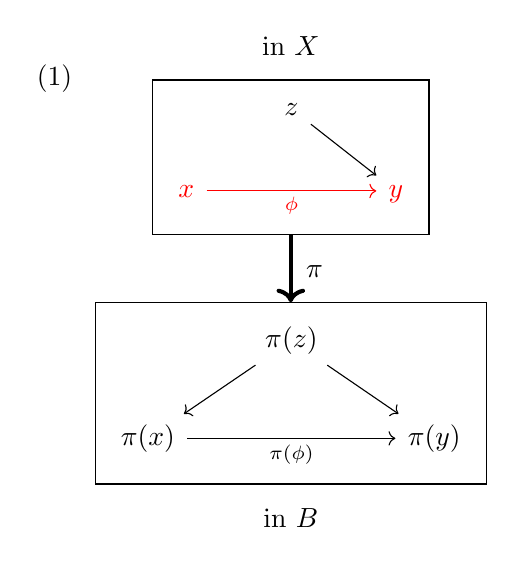
\begin{tikzpicture}[mybox/.style={draw, inner sep=5pt}]
        \node[mybox] (X) at (0,3){%
            \begin{tikzcd}
                {} & z \ar[rd]& {} \\
                \color{red}x \ar[rr, red, "\phi"'] &{}& \color{red}y
            \end{tikzcd}
        };
        \node[mybox] (B) at (0,0){%
            \begin{tikzcd}
                {} & \pi(z) \ar[rd]\ar[ld]& {} \\
                \pi(x) \ar[rr, "\pi(\phi)"'] &{}& \pi(y)
            \end{tikzcd}
        };

        \node [above=5pt of X] {in $\cat{X}$};
        \node [below=5pt of B] {in $\cat{B}$};
        \draw [->, line width=1.5pt] (X) edge (B);
        \node at (0.3,1.55) {$\pi$};
        %% \draw (3.5,4) -- (3.5,-1);
        \node at (-3,4) {($1$)};
        \end{tikzpicture}
        \qquad
        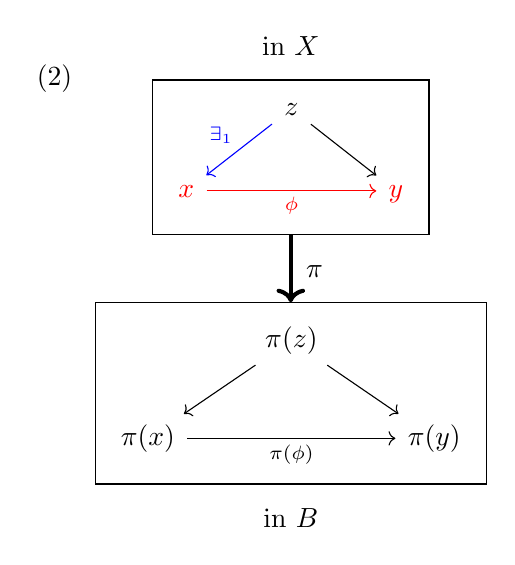
\begin{tikzpicture}[mybox/.style={draw, inner sep=5pt}]
        \node[mybox] (X) at (0,3){%
            \begin{tikzcd}
                {} & z \ar[rd] \ar[ld, blue, "\exists_1"']& {} \\
                \color{red}x \ar[rr, red, "\phi"'] &{}& \color{red}y
            \end{tikzcd}
        };
        \node[mybox] (B) at (0,0){%
            \begin{tikzcd}
                {} & \pi(z) \ar[rd]\ar[ld]& {} \\
                \pi(x) \ar[rr, "\pi(\phi)"'] &{}& \pi(y)
            \end{tikzcd}
        };

        \node [above=5pt of X] {in $\cat{X}$};
        \node [below=5pt of B] {in $\cat{B}$};
        \draw [->, line width=1.5pt] (X) edge (B);
        \node at (0.3,1.55) {$\pi$};
        \node at (-3,4) {($2$)};
        \end{tikzpicture}
        \end{center}
        %% }}}

    \item
        $y \in \cat{X}, \phi \colon u \to \pi(y) \in \cat{B}$に対し,
        以下の図式を満たす
        \tablefootnote{すなわち,$\pi(x)=u, \pi(x \to y)=u \to \pi(y)$を満たす.}
        \underline{$x \in \cat{X}$とデカルト射$x \to y \in \cat{X}$}を,
        $u \to \pi(y)$のデカルト持ち上げ (cartesian lifting) と呼ぶ.
        % {{{
        \begin{center}
        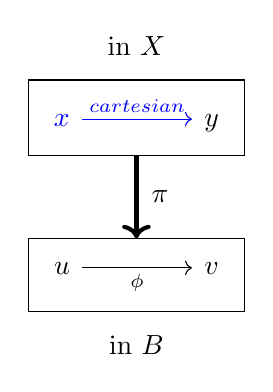
\begin{tikzpicture}[mybox/.style={draw, inner sep=5pt}]
        \node[mybox] (X) at (0,2){%
        \begin{tikzcd}[column sep=40pt]
            \color{blue}x \ar[r, blue, "\text{cartesian}"]& y
        \end{tikzcd}
        };
        \node[mybox] (B) at (0,0){%
        \begin{tikzcd}[column sep=40pt]
            u \ar[r, "\phi"']& v
        \end{tikzcd}
        };

        \node [above=5pt of X] {in $\cat{X}$};
        \node [below=5pt of B] {in $\cat{B}$};
        \draw [->, line width=1.5pt] (X) edge (B);
        \node at (0.3,1) {$\pi$};
        \end{tikzpicture}
        \end{center}
        %% }}}
        デカルト持ち上げで得られる対象(ここでの$x$)を$\phi^*y$と書く.

    \item
        任意の$y \in \cat{X}$と$\cat{B}$の射$u \to \pi(y)$に対してデカルト射が存在する
        関手$\pi \colon \cat{X} \to \cat{B}$を$\cat{B}$へのファイブレーション (fibration) という.

    \item
        $\pi \colon \cat{X} \to \cat{B}$をファイブレーションとする時,
        $\cat{X}$はファイバー圏 (fibered category)と呼ぶ.

    \item
        $\pi \colon \cat{X} \to \cat{B}$をファイブレーションとする時,
        部分圏$\cat{X}' \subset \cat{X}$が部分ファイバー圏であるとは,
        $\pi$の$\cat{X}'$への制限がファイブレーションであり,
        かつ$\cat{X}'$でのデカルト射は$\cat{X}$でもデカルト射であるということ.

    \item
        $\pi \colon \cat{X} \to \cat{B}$をファイブレーションとする時,
        $x$が$\cat{X}$の対象で$y=\pi(x)$ならば,$x$は$y$上の対象であるという.
        $\phi$が$\cat{X}$の射で$\psi=\pi(x)$ならば,$\phi$は$\psi$上の射であるという.
    \end{enumerate}
    \end{Def}

    ファイブレーションはファイバー積の一般化として考案された.
    このことは次の例を見れば分かるだろう.

    \begin{Example}[\cite{FGAexp} chapter 3]\label{example:c_arrows}
        圏$\cat{C}$に対し,圏$\cat{C}^{\to}$を次のように定義する.
        \begin{description}
            \item[\underline{対象}] \mnewline
                圏$\cat{C}$の射.$[\, x \to u \,]$のように書く.

            \item[\underline{射}] \mnewline
            射$[x \to u] \to [y \to v]$は
            次の図式を可換にする$2$つの射$x \to y, u \to v$の組. 
            \[
            \begin{tikzcd}
                x \ar[r, dashed]\ar[d]& y \ar[d]\\
                u \ar[r, dashed]& v
            \end{tikzcd}
            \]
        \end{description}

        関手$p \colon \cat{C}^{\to} \to \cat{C}$を$[\, x \to y \,] \mapsto y$のように定める.
        圏$\cat{C}$がファイバー積(デカルト積)と持つならば,
        それによって$p$はファイブレーションと成る.
        三角持ち上げはファイバー積の普遍性から得られる.
    \end{Example}

    以下の例は表現可能関手に対応する(後述する)ものであり,重要である.
    \begin{Example}\label{example:rep_fibration}
        任意の圏$\cat{B}$と任意の対象$b \in \cat{B}$に対し,
        関手$\cat{B}/b \to \cat{B}$を$[\, x \to b \,] \mapsto x$と定義する.
        この関手はファイブレーションである.
        デカルト持ち上げは射の合成で与えられ,
        三角持ち上げはスライス圏$\cat{B}/b'$の射の定義から自明に得られる.
    \end{Example}
    
    その他の具体例は \cite{FGAexp} chapter 3 に多く掲載されている.

    \begin{Def}[ファイブレーションの射]
        圏$\cat{B}$への$2$つのファイブレーション
        $\pi \colon \cat{X} \to \cat{B}, \rho \colon \cat{Y} \to \cat{B}$を考える.
        
    \begin{enumerate}
        \item
            関手$F \colon \cat{X} \to \cat{Y}$を考える.
            関手$F$が$\pi=\rho \circ F$を満たし,かつデカルト射をデカルト射へ写す時,
            関手$F$をファイブレーション$\pi, \rho$の射と呼ぶ.

        \item
            $\cat{B}$へのファイブレーションとその射が成す圏を$\Fib{B}$とする.

        \item
            二つのデカルト関手$F,G \colon \cat{X} \to \cat{Y}$と,
            その間の自然変換$\eta \colon F \to G$を考える.
            \begin{center}
            \begin{tikzcd}[column sep=3cm]
                \cat{X} \ar[rd, "\pi"]
                    \ar[dd, shift right=3mm, "F"'{name=F}] \ar[dd, shift left=3mm, "G"{name=G}]& {} \\
                {} & \cat{B} \\
                \cat{Y} \ar[ru, "\rho"']& {}
                \ar[Rightarrow, from=F, to=G, shorten >=2pt, shorten <=2pt, "\eta"]
            \end{tikzcd}
            \end{center}
            任意の$x \in \cat{X}$について,
            $\rho(\eta_x) \colon \rho(F(x)) \to \rho(G(x))$が恒等射になるとき,
            $\eta$は基底を保つ自然変換 (base-preserving natural transformation) であるという.

        \item
            $\HOM_{/\cat{B}}(\cat{X}, \cat{Y})$あるいは$\HOM_{/\cat{B}}(\pi, \rho)$を,
            ファイブレーション$\pi, \rho$の射と基底を保つ自然変換が成す圏とする.

        \item
            ファイブレーション$\pi, \rho$が同値であるとは,
            $2$つの射$F \colon \cat{X} \rightleftarrows \cat{Y} \colon G$が存在し,
            $G \circ F$と$\id[\cat{X}]$,$F \circ G$と$\id[\cat{Y}]$の間に
            基底を保つ自然同型が存在すること.
    \end{enumerate}
    \end{Def}
    以下,ファイブレーションの射の間の射と言えば基底を保つ自然変換のことである.

    \begin{Remark}
        ファイブレーションの圏$\Fib{B}$は圏の圏であるから,
        $2$圏と呼ばれる種類の圏である.
        この論文では少し$2$圏の用語を用いるが,説明を省略する.

        また,以下でファイブレーションの圏$\Fib{B}$における図式が可換であるとは,
        それが$2$可換であることを意味する.
        すなわち,$\Fib{B}$における以下のような図式が可換であるとは,
        射(関手)$f \circ s$と$g \circ t$の間に基底を保つ自然同型が存在するということである.
        \[
        \begin{tikzcd}
            \cat{X} \ar[r, "s"]\ar[d, "t"']& \cat{Y} \ar[d, "f"]\\
            \cat{Z} \ar[r, "g"']& \cat{W}
        \end{tikzcd}
        \]
    \end{Remark}

    \begin{Prop}[\cite{FGAexp} chapter 5]\nocite{Vistoli07}
    \begin{myenum}
    \item
        デカルト射の合成はデカルト射である.
    \item
        ファイブレーション$\pi \colon \cat{X} \to \cat{B}$を考える.
        $\cat{X}$の射$\phi \colon x \to y, \psi \colon y \to z$について,
        射$\psi \circ \phi, \psi$がデカルト射ならば$\psi$もデカルト射.
    \end{myenum}
    \end{Prop}
    \begin{proof}
        三角持ち上げのみを用いて証明できる.
        簡単なので証明は省略する.
    \end{proof}

    次の命題の証明はデカルト持ち上げと三角持ち上げの使い方をよく示している.
    \begin{Prop}
        $\pi \colon \stX \to \cat{B}$をファイブレーションとする.
        $\stX$の射$x \to y$は以下のような二つの射の合成$x \to z \to y$に分解できる.
        \begin{itemize}
            \item 恒等射$\id[\pi(x)]$上の射$x \to z$,
            \item 射$\pi(x \to y)$上のデカルト射$z \to y$.
        \end{itemize}
    \end{Prop}
    %% {{{
    \begin{proof}
        $\pi(\phi)$のデカルト持ち上げとして以下の図式(1)の$z$と$z \to y$を得る.
        さらに三角持ち上げにより図式(2)の通り$\id[\pi(x)]$上の射$x \to z$を得る.
        \begin{center}
        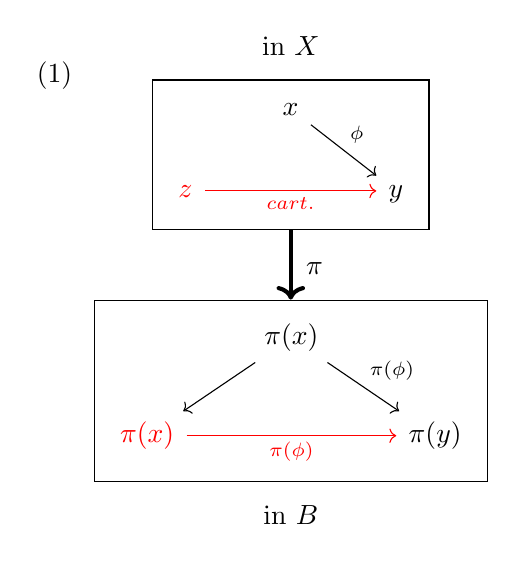
\begin{tikzpicture}[mybox/.style={draw, inner sep=5pt}]
        \node[mybox] (X) at (0,3){%
            \begin{tikzcd}
                {} & x \ar[rd, "\phi"]& {} \\
                \color{red}z \ar[rr, red, "\text{cart.}"']&{}& y
            \end{tikzcd}
        };
        \node[mybox] (B) at (0,0){%
            \begin{tikzcd}
                {} & \pi(x) \ar[rd, "\pi(\phi)"]\ar[ld, "\id"']& {} \\
                \color{red}\pi(x) \ar[rr, red, "\pi(\phi)"'] &{}& \pi(y)
            \end{tikzcd}
        };

        \node [above=5pt of X] {in $\cat{X}$};
        \node [below=5pt of B] {in $\cat{B}$};
        \draw [->, line width=1.5pt] (X) edge (B);
        \node at (0.3,1.55) {$\pi$};
    %    \draw (4,4) -- (4,-1);
        \node at (-3,4) {($1$)};
        \end{tikzpicture}
        \qquad \qquad
        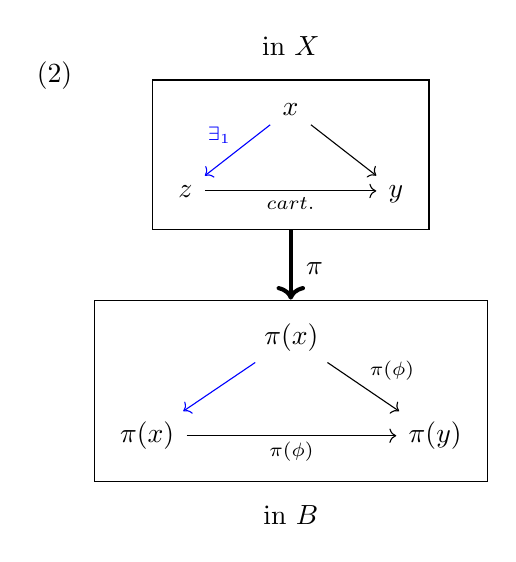
\begin{tikzpicture}[mybox/.style={draw, inner sep=5pt}]
        \node[mybox] (X) at (0,3){%
            \begin{tikzcd}
                {} & x \ar[rd] \ar[ld, blue, "\exists_1"']& {} \\
                z \ar[rr, "\text{cart.}"'] &{}& y
            \end{tikzcd}
        };
        \node[mybox] (B) at (0,0){%
            \begin{tikzcd}
                {} & \pi(x) \ar[rd, "\pi(\phi)"]\ar[ld, blue, "\id"']& {} \\
                \pi(x) \ar[rr, "\pi(\phi)"'] &{}& \pi(y)
            \end{tikzcd}
        };

        \node [above=5pt of X] {in $\cat{X}$};
        \node [below=5pt of B] {in $\cat{B}$};
        \draw [->, line width=1.5pt] (X) edge (B);
        \node at (0.3,1.55) {$\pi$};
        \node at (-3,4) {($2$)};
        \end{tikzpicture}
        \end{center}
    \end{proof}
    %%}}}

    \begin{Prop}\label{prop:iso_over_iso}
        $\pi \colon \cat{X} \to \cat{B}$をファイブレーションとする.
        $\cat{X}$の任意のデカルト射$\phi \colon x \to y$について,
        $\phi$が同型射であることと$\Phi:=\pi(\phi)$が同型射であることは同値.
    \end{Prop}
    %% {{{
    \begin{proof}
        以下の図式(1)に三角持ち上げを用いれば,
        $\phi \circ \psi=\id[y]$なる射$\psi \colon y \to x$を得る.
        さらに図式(2)に於いて,
        $\phi \circ \id[x]=\phi=\phi \circ \psi \circ \phi$と三角持ち上げの一意性から
        $\psi \circ \phi=\id[x]$を得る.
        \begin{center}
        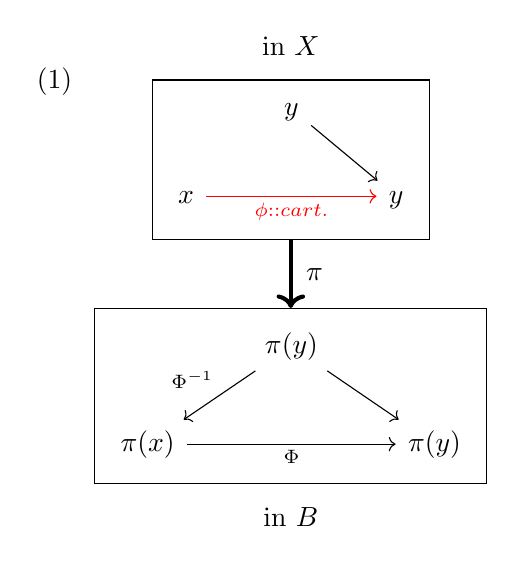
\begin{tikzpicture}[mybox/.style={draw, inner sep=5pt}]
        \node[mybox] (X) at (0,3){%
            \begin{tikzcd}
                {} & y \ar[rd, "\id"]& {} \\
                x \ar[rr, red, "\phi\text{ :: cart.}"']&{}& y
            \end{tikzcd}
        };
        \node[mybox] (B) at (0,0){%
            \begin{tikzcd}
                {} & \pi(y) \ar[rd, "\id"]\ar[ld, "\Phi^{-1}"']& {} \\
                \pi(x) \ar[rr, "\Phi"'] &{}& \pi(y)
            \end{tikzcd}
        };

        \node [above=5pt of X] {in $\cat{X}$};
        \node [below=5pt of B] {in $\cat{B}$};
        \draw [->, line width=1.5pt] (X) edge (B);
        \node at (0.3,1.55) {$\pi$};
    %    \draw (4,4) -- (4,-1);
        \node at (-3,4) {($1$)};
        \end{tikzpicture}
        \qquad \qquad
        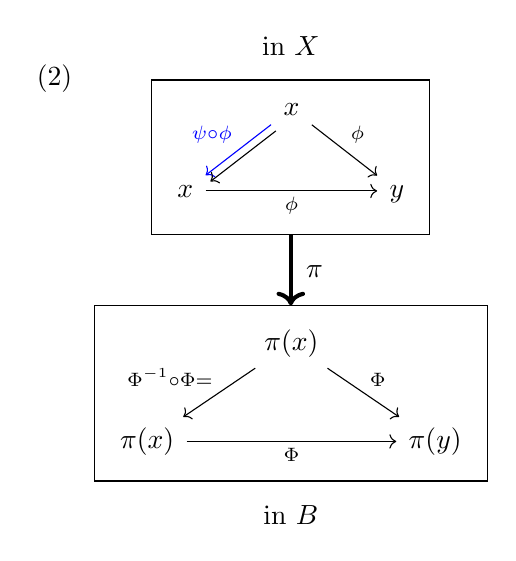
\begin{tikzpicture}[mybox/.style={draw, inner sep=5pt}]
        \node[mybox] (X) at (0,3){%
            \begin{tikzcd}
                {} & x \ar[ld, blue, "\psi \circ \phi"'] \ar[ld, shift left=1mm, "\id"] \ar[rd, "\phi"]& {} \\
                x \ar[rr, "\phi"'] &{}& y
            \end{tikzcd}
        };
        \node[mybox] (B) at (0,0){%
            \begin{tikzcd}
                {} & \pi(x) \ar[ld, "\Phi^{-1} \circ \Phi=\id"']\ar[rd, "\Phi"]& {} \\
                \pi(x) \ar[rr, "\Phi"'] &{}& \pi(y)
            \end{tikzcd}
        };

        \node [above=5pt of X] {in $\cat{X}$};
        \node [below=5pt of B] {in $\cat{B}$};
        \draw [->, line width=1.5pt] (X) edge (B);
        \node at (0.3,1.55) {$\pi$};
        \node at (-3,4) {($2$)};
        \end{tikzpicture}
        \end{center}
    \end{proof}
    %% }}}

    \begin{Remark}\label{remark:cleavage}
        ファイブレーション $\pi \colon \cat{X} \to \cat{B}$を考える.
        $\cat{X}$の任意の対象$x$と$\cat{B}$の射$\phi \colon b' \to \pi(x)$に対し,
        異なるデカルト持ち上げが二つ以上存在しうることに注意して欲しい.
        したがって「射$\phi$のデカルト持ち上げを$f$とする」という時,
        我々はデカルト射$f \colon \phi^*x \to x$を\underline{選び取っている}.
        この選択を$\pi$の裂開 (cleavage)
        \footnote
        {
            この用語は和訳が定まっていないが,
            「力ずくで割ったもの」「自然に任せて裂き割ったもの」というニュアンスだと筆者は考える.
            『新英和中辞典』(研究社)では
            「(おのなどで木目・劈開(へきかい)面にそって)裂く,割る」
            「〈道を〉切り開いて(…を)進む」「かき分けて進む」
            などの訳が与えられている.
        }
        と呼ぶ.
        クラスを用いた厳密な定義は\cite{FGAexp} 第$3$章を参照せよ.
        選択公理から,任意の$\pi, x, \phi$についてその裂開が存在する.

        裂開のとり方によっては以下で定義するファイバー$\cat{X}(-)$が関手にならない.
        しかし,任意のファイブレーション$\pi$に対して,
        $\pi$と同値なファイブレーション$\tilde{\cat{X}} \to \cat{B}$と
        ファイバー$\tilde{\cat{X}}(-)$が関手に成る裂開の組が存在する(\cite{FGAexp} 第$3$章).
        このようなファイブレーションと裂開の組は``split fibration"と呼ばれる.
        ここでファイバー$\tilde{\cat{X}}(-)$が関手に成るということを言い換えれば,
        デカルト持ち上げを2回繰り返して得られる$\phi^*\psi^*x$と
        一度にデカルト持ち上げした$(\psi \circ \phi)^*x$が等しい ($\phi^*\psi^*x=(\psi \circ \phi)^*x$)
        ということである.
        また,以下での議論はファイブレーションをそれと同値なファイブレーションに
        取り替えても変わらないものである.
        なので最初からこのようなファイブレーションと裂開をとっていると考え,
        一々裂開に言及しない.
    \end{Remark}

    ファイブレーションと前層は一方から他方が構成できる関係に有る.
    しかもこの構成操作の組は互いに逆操作である.

    \begin{Def}[ファイバー圏のファイバー; fiber of fibered category]
        ファイブレーション $\pi \colon \cat{X} \to \cat{B}$を考える.

        任意の$\cat{B}$の対象$b \in \cat{B}$について,
        以下で定める圏を$\cat{X}(b)$と書く.
        \begin{description}[labelindent=0.5cm]
            \item[\underline{対象}] $\pi(x)=b$となる$\cat{X}$の対象$x$.
            \item[\underline{射}] $\pi(\phi)=\id[b]$となる$\cat{X}$の射$\phi$.
        \end{description}
        したがって$\cat{X}(b)$は$\cat{X}$の部分圏である.

        圏$\cat{B}$の射$\phi \colon b' \to b$に対し,
        射$\cat{X}(\phi) \colon \cat{X}(b) \to \cat{X}(b')$を次で定める.
        \begin{defmap}
            \cat{X}(\phi)\colon & \cat{X}(b)& \to& \cat{X}(b') \\
            \textbf{\underline{対象}}& x& \mapsto& \phi^*x \\
            \textbf{\underline{射}}& \alpha \colon x \to y & \mapsto&
            \left(
                \parbox{4.3cm}
                {
                    $\alpha \circ \bar{\phi}^{x} \colon \phi^*x \to y$と \\
                    $\bar{\phi}^{y} \colon \phi^* y \to y$から \\
                    三角持ち上げで誘導される射
                }
            \right)
%            \begin{array}{l}
%                \text{$\alpha \circ \lift_{x} \phi \colon \phi^*x \to y$と} \\
%                \text{$\lift_{y} \phi \colon \phi^* y \to y$から} \\
%                \text{三角持ち上げで誘導される射}
%            \end{array}
        \end{defmap}
        ここで$\bar{\phi}^{x} \colon \phi^*x \to x, \bar{\phi}^{y} \phi \colon \phi^* y \to y$は
        それぞれ$\phi$と$x$,$\phi$と$y$に関するデカルト持ち上げである.

        ファイブレーションの射$f \colon \cat{X} \to \cat{G}$と$b \in \cat{B}$に対し,
        $f$を部分圏$\cat{X}(b)$に制限することで得られる射を
        $f_{b} \colon \cat{X}(b) \to \cat{G}(b)$と書く.
    \end{Def}
    
    \begin{Remark}
    標語的には次のように定義されている.
    \[
        \stX_b=\stX(b) := \text{``}
        \pi^{-1} \left(
        \begin{tikzcd}
            b \arrow[loop, distance=2em, in=325, out=35, "\id"]
        \end{tikzcd}
    \right)\text{"}
    \]
    \end{Remark}

    \begin{Def}[Grothendieck 構成; Grothendieck construction]
        関手$F \colon \opcat{\cat{B}} \to \Cat/\cat{B}$について,
        以下のように圏$\int F$を定義する.
        \begin{description}[labelindent=1cm]
            \item[\underline{対象}] $b \in \cat{B}$と$x \in F(b)$の組$(b, x)$.
            \item[\underline{射}] $\phi \colon b \to b'$と$\Phi \colon F(\phi)(x) \to x'$の組$(\phi, \Phi)$.
        \end{description}
        射の合成は$(\psi, \Psi) \circ (\phi, \Phi)=(\psi \circ \phi, \Phi \circ F(\psi)(\Phi))$で与えられる.
        この圏によって以下の関手が定まる.
        \begin{defmap}
            \int \colon & \Hom_{\Cat}(\opcat{\cat{B}}, \Cat/\cat{B})& \to& \Fib{B} \\
            {}& F& \mapsto& \int F
        \end{defmap}
    \end{Def}
    この構成$\int F$は要素の圏 (the category of elements) とも呼ばれている.

    \begin{Example}
        スキーム$S$について,
        表現可能関手$\ftor{S}:=\Hom_{\Sch}(-, S)$は Grothendieck 構成によって$\Sch/S$に対応する.
        これは例(\ref{example:rep_fibration})で触れたものである.
    \end{Example}

    \begin{Lemma}[\cite{Olsson16} Prop 3.2.8]
        Grothendieck 構成$\int$は狭義$2$同値 (strict $2$-equivalence) を与える.
        逆はファイバーを取る操作である.
    \end{Lemma}
    したがって関手の理論とsplit fibration(注意(\ref{remark:cleavage}))の理論は互いに翻訳できる.

    以下ではしばしば暗黙のうちに Grothendieck 構成を用い,
    層をファイブレーションとして扱う.
    特にスキーム$X$とファイバー圏$\Sch/X$は同じ記号で書く.

    \begin{Lemma}[$2$米田の補題; $2$-Yoneda Lemma, Fibered Yoneda Lemma]
        $\pi \colon \stX \to \cat{B}$をファイブレーションとする.
        以下のように関手を定める.
        \begin{defmap}
            Y\colon & \cat{B}& \to& \Fib{B}\\
            {}& b& \mapsto& \cat{B}/b
        \end{defmap}
        例(\ref{example:rep_fibration})で触れたとおり,
        $\cat{B}/b \to \cat{B}$は確かにファイブレーションであることに注意.
        この時,圏同値$\HOM_{/\cat{B}}(Y(b), \stX) \simeq \stX(b)$が成り立つ.
    \end{Lemma}

    \begin{Def}[亜群のファイバー圏; category fibered in groupoids]
        ファイブレーション$\cat{X} \to \cat{B}$について,
        圏$\cat{X}$の全ての射がデカルト射であるとき,
        ファイバー圏$\cat{X}$を亜群のファイバー圏という.
    \end{Def}

    \begin{Lemma}
        ファイブレーション$\cat{X} \to \cat{B}$を考える.
        $\cat{X}$が亜群のファイバー圏であることと,
        任意の$b \in \cat{B}$に対してファイバー$\cat{X}(b)$は亜群であることは同値である
    \end{Lemma}
    \begin{proof}
        一般に,同型射上のデカルト射は同型射である(命題(\ref{prop:iso_over_iso})).
        $\cat{X}$が亜群のファイバー圏ならば
        ファイバー$\cat{X}(b)$の射は恒等射$\id[b]$上のデカルト射だから,
        補題が成り立つ.
        逆は容易.\cite{SP} 003Vにも証明が有る.
    \end{proof}

\subsection{スタック}
    層の一般化としてスタックを定義する.

    記法を定める.
    $\cat{C}$を景,
    $\pi \colon \stF \to \cat{C}$をファイブレーションとする.
    対象$U \in \cat{C}$と
    その被覆$\covU=\{\phi_i \colon U_i \to U\}_{i \in I} \in \Cov(U)$について,
    \[ U_{ij}:=U_i \times_U U_j, \quad U_{ijk}:=U_i \times_U U_j \times_U U_k \ \ \ (i,j,k \in I) \]
    と書くことにする.
    また,添字$a,b=i \mor j \mor k$について,
    ファイバー積からの射影を
    \[ \pr_{a} \colon U_{ij} (\mor U_{ijk}) \to U_{a}, \qquad \pr_{a,b} \colon U_{ijk} \to U_{ab} \]
    とする.
    さらに$\pr_{i} \colon U_{ij} \to U_{i}$による引き戻しを$(-)|_{U_{ij}}$などと書く.

    \begin{Def}[降下データ; descent data]
    $\cat{C}$を景,
    $\pi \colon \stF \to \cat{C}$をファイブレーションとする.

    $\cat{C}$の対象$U$とその被覆$\covU=\{\phi_i \colon U_i \to U\}_{i \in I} \in \Cov(U)$に対し,
    圏$\stF(\covU)$を次のように定める.
    \begin{description}
        \item[\underline{対象}] \hfill \vspace{-0.2cm}
            \begin{itemize}
                \item $\xi_i \in \stF(U_i)$なる対象のクラス $\{\xi_i\}_{i \in I}$と,
                \item
                    $\stF(U_{ij})$中の同型射$\sigma_{ij} \colon \xi_j|_{U_{ij}} \to \xi_i|_{U_{ij}}$の
                    クラス $\{\sigma_{ij}\}_{i,j \in I}$
            \end{itemize}
            の組$(\{\xi_i\}, \{\sigma_{ij}\})$であって,
            以下で述べるコサイクル条件を満たすもの.
            このような組を降下データつき対象と呼ぶ.
            特に,同型からなるクラス $\{\sigma_{ij}\}$が降下データと呼ばれる.

        \item[\underline{射}] \mnewline
            射$\{\alpha_i\} \colon (\{\xi_i\}, \{\sigma_{ij}\}) \to (\{\eta_i\}, \{\tau_{ij}\})$とは,
            $\stF(U_i)$の射$\alpha_i \colon \xi_i \to \eta_i$の集合であって,\mnewline
            $\sigma_{ij}, \tau_{ij}$と整合的であるもの.
            すなわち,任意の$i, j \in I$について以下の図式が可換であるもの.
            \[
            \begin{tikzcd}
                \xi_j|_{U_{ij}} \ar[d, "\sigma_{ij}"'] \ar[r, "\alpha_j|_{U_{ij}}"]& \eta_j|_{U_{ij}} \ar[d, "\tau_{ij}"]\\
                \xi_i|_{U_{ij}} \ar[r, "\alpha_i|_{U_{ij}}"']& \eta_i|_{U_{ij}}
            \end{tikzcd}
            \]
    \end{description}

    \step{コサイクル条件}
    組$(\{\xi_i\}, \{\sigma_{ij}\})$がコサイクル条件を満たすとは,
    任意の$i,j,k \in I$について以下が成り立つということ.
    \[ \sigma_{ik}|_{U_{ijk}}=(\sigma_{ij}|_{U_{ijk}}) \circ (\sigma_{jk}|_{U_{ijk}}). \]
    図式でかけば,圏$\stF(U_{ijk})$における以下の図式が可換であることと同値.
    \[
    \begin{tikzcd}[row sep=70pt]
        \xi_k|_{U_{ijk}} \ar[rd, "\sigma_{ik}|_{U_{ijk}}"'] \ar[rr, "\sigma_{jk}|_{U_{ijk}}"]
            & {}
            & \xi_j|_{U_{ijk}} \ar[ld, "\sigma_{ij}|_{U_{ijk}}"] \\
        {} & \xi_i|_{U_{ijk}} & {}
    \end{tikzcd}
    \]
    \end{Def}

    \begin{Remark}
        この定義に於いて$U_{ij}, U_{ijk}$を暗黙のうちに選択しているが,
        どのように選択しても得られる圏は同型に成る.
        $U_{ij}, U_{ijk}$の選択も込めて
        $(\{\xi_i\}, \{\xi_{ij}\}, \{\xi_{ijk}\})$を$\stF(\covU)$の対象とする
        定義の仕方も有る.詳細は\cite{FGAexp}を参照して欲しい.
    \end{Remark}

    \begin{Def}
        $\cat{C}$を景,
        $\pi \colon \stF \to \cat{C}$をファイブレーションとする.
        対象$U \in \cat{C}$と
        その被覆$\covU=\{\phi_i \colon U_i \to U\}_{i \in I} \in \Cov(U)$について,
        $\stF(\covU)$の元を以下のデータに対応させる:
        \begin{itemize}
            \item $\xi_i:=\phi_i^*\xi$のクラス $\{\xi_i\}_{i \in I}$.
            \item
                恒等射の集合$\{ \id \colon \xi_j|_{U_{ij}} \to \xi_i|_{U_{ij}} \}_{i,j}$
                標準的同型のクラス $\{ \sigma_{ji} \colon \xi_j|_{U_{ij}} \to \xi_i|_{U_{ij}} \}_{i,j}$.
        \end{itemize}
        $\xi_i|_{U_{ij}}$と$\xi_j|_{U_{ij}}$は
        いずれも
        \[ \phi_i \circ \pr_i=\phi_j \circ \pr_j \colon U_{ij} \to U \]による$\xi$の引き戻し
        であるから注意(\ref{remark:cleavage})より等しいことに注意せよ.
        このデータをまとめて$(\{\phi_i^*\xi\}, \mathrm{cano})$などと書く.
        この対応を$\epsilon_{\covU} \colon \stF(U) \to \stF(\covU)$と書く.
        この対応は関手と成る.
    \end{Def}

    \begin{Def}[スタック; stack]
        $\cat{C}$を景,
        $\pi \colon \stF \to \cat{C}$をファイブレーションとする.
        任意の対象$U \in \cat{C}$と
        その任意の被覆$\covU=\{\phi_i \colon U_i \to U\}_{i \in I} \in \Cov(U)$について
        関手$\epsilon_{\covU} \colon \stF(U) \to \stF(\covU)$が圏同値を与える時,
        $\stF$をスタックと呼ぶ.
        スタックの射はファイバー圏としての射である.
        景$\cat{C}$上のスタックの圏を$\St{C}$と書く.
    \end{Def}

    \begin{Example}
        ファイブレーション $\shF \to \Set$ について$\shF$がスタックであることと,
        $\shF$のファイバーが(集合の)層であることは同値である.
    \end{Example}

    \begin{Def}
        $\cat{C}$を景,
        $\pi \colon \stF \to \cat{C}$をファイブレーションとする.
        $\stF$が亜群のファイバー圏で,かつスタックである時,
        $\stF$を亜群のスタックという.
        亜群のスタックの射はファイバー圏としての射である.
        景$\cat{C}$上の亜群のスタックの圏を$\GrSt{C}$と書く.
    \end{Def}
    
    \begin{Prop}\label{prop:St_GrSt_has_fibprod}
        任意の景$\cat{C}$について,
        スタックの圏$\St{C}$と
        亜群のスタックの圏$\GrSt{C}$はファイバー積を持つ.
    \end{Prop}
    \begin{proof}
        $\St{C}$の射$F \colon \stX \to \stZ$と$F \colon \stY \to \stZ$をとり,
        $F, G$のファイバー積を構成する.
        ファイバー積の構成とファイブレーションの存在だけ示し,
        実際にファイバー積であることや,
        (亜群の)スタックのファイバー積が(亜群の)スタックに成ることの証明は省略する.

        \step{圏$\cat{P}$の構成}
        圏$\cat{P}$を以下のように定義する.
        \begin{description}
            \item[\underline{対象}]
                以下の$4$つ組
                \begin{itemize}
                    \item 対象$b \in \cat{B}$,
                    \item 対象$x \in \stX(b)$と$y \in \stY(b)$,
                    \item $\stZ$の恒等射上の同型射$\alpha \colon Fx \to Gy$.
                \end{itemize}
            
            \item[\underline{射}] \mnewline
                射$(b, x, y, \alpha) \to (b', x', y', \alpha')$は,
                二つの射$\phi_{\stX} \colon x \to x', \phi_{\stY} \colon y \to y'$であって以下を満たすもの:
                $\phi_{\stX}, \phi_{\stY}$は同じ射$b' \to b$上の射で,
                以下の可換図式を満たすもの.
                \[
                \begin{tikzcd}
                    Fx \ar[d, red, "F\phi_{\stX}"']\ar[r, "\alpha"]& Gy \ar[d, red, "G\phi_{\stY}"]\\
                    Fx' \ar[r, "\alpha'"']& Gy'
                \end{tikzcd}
                \]
        \end{description}

        \step{$\cat{P}$でのデカルト持ち上げ}
        この圏は$\pi \colon (b,x,y,\alpha) \mapsto b$によってファイバー圏になることを示す.
        $f \colon b' \to b$の$\xi=(b, x, y, \alpha)$に関する
        デカルト持ち上げ$\chi_{\xi} \colon f^*\xi \to \xi$は次のように定義される.
        \[
            \chi_{\xi}=(f^*x \xrightarrow{\chi_x} x, f^*y \xrightarrow{\chi_y} y)
            \colon
            f^*\xi=(b', f^*x, f^*y, \bar{\alpha}) \to \xi.
        \]
        ここで$\chi_x \colon f^*x \to x$は$f$の$x$に関するデカルト持ち上げである.
        $\chi_y$も同様.
        さらに$\bar{\alpha}$は以下の三角持ち上げで得られる射である
        \footnote
        {
            $f^*\alpha \colon f^*Fx \to f^*Gy$とは異なる.
            同型$Ff^*x \to F^*Fx, Gf^*y \to f^*Gy$と$f^*\alpha \colon Fx \to Gy$を
            合成しても$\bar{\alpha}$は得られる.
        }.
        \begin{center}
        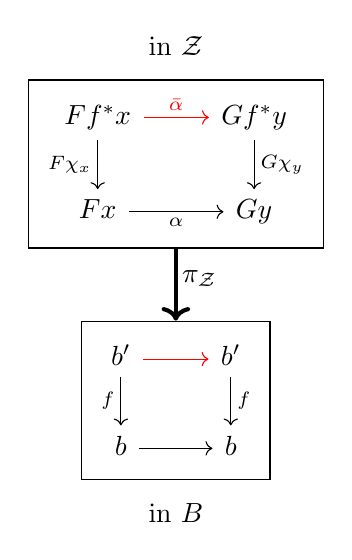
\begin{tikzpicture}[mybox/.style={draw, inner sep=5pt}]
        \node[mybox] (X) at (0,3){%
            \begin{tikzcd}
                Ff^*x \ar[d, "F\chi_x"']\ar[r, red, "\bar{\alpha}"]& Gf^*y \ar[d, "G\chi_y"]\\
                Fx \ar[r, "\alpha"']& Gy
            \end{tikzcd}
        };
        \node[mybox] (B) at (0,0){%
            \begin{tikzcd}
                b' \ar[d, "f"']\ar[r, red, "\id"]& b' \ar[d, "f"]\\
                b \ar[r, "\id"]& b
            \end{tikzcd}
        };

        \node [above=5pt of X] {in $\stZ$};
        \node [below=5pt of B] {in $\cat{B}$};
        \draw [->, line width=1.5pt] (X) edge (B);
        \node at (0.3,1.55) {$\pi_{\stZ}$};
        \end{tikzpicture}
        \end{center}
        ファイバー圏の射はデカルト射を保つので$F\chi_x, G\chi_y$もデカルト射.
        したがって三角持ち上げが出来る.
        $\bar{\alpha}$が同型であることは三角持ち上げの一意性を用いて容易に証明できる.
        また,この可換図式から$\chi_{\xi}$が$\cat{P}$の射であることも分かる.
    \end{proof}

\section{代数的空間}
    この節では\cite{Olsson16}と\cite{SP}を参考としてほしい.

\subsection{表現可能な層/射}
    この節ではスキーム$S$を固定し,
    $S$の fppf 大景$\FPPF(S)$上の層
    \footnote{ fppf 大景$\ET(S)$上の層は「空間 (space)」と呼ばれるが,紛らわしいので本論文では使わない. }
    を考える.
    これは(表現可能な)層$S$への射を持つことに注意.

    \begin{Lemma}[\cite{Olsson16} Theorem 4.1.2]\label{lemma:rep_functor_is_fppf_sheaf}
        $X$をスキーム$S$上のスキームとする.
        表現可能関手$\Hom_{\Sch/S}(-,X)$は
        fppf 大景$\FPPF(S)$上の層である.
    \end{Lemma}
    
    以下,スキーム$X$と表現可能関手$\Hom(-,X)$を同じ記号で書く.

    \begin{Def}[表現可能な層/層の射]
    \begin{myenum}
    \item
        fppf 大景$\FPPF(S)$上の層$F$があるスキーム$X$と層として同型である時,
        $F$は(スキーム$X$によって)表現可能であるという.

    \item
        $\FPPF(S)$上の層の射$f \colon X \to Y$が表現可能であるとは,
        スキームからの任意の射$U \to Y$に対し,
        ファイバー積$U \times_{Y} X$が表現可能であるということ.
    \end{myenum}
    \end{Def}
    
    \begin{Def}[表現可能な層/層の射の性質]
    \begin{myenum}
    \item
        fppf 大景$\FPPF(S)$上の層$F$がスキーム$X$で表現可能な時,
        層$F$が性質$\mathcal{P}$を持つとは,
        スキーム$X$が性質$\mathcal{P}$を持つということである.
    \item
        $\FPPF(S)$上の層の射$f \colon X \to Y$が表現可能である時,
        層の射$f$が性質$\mathcal{P}$を持つとは,
        スキームからの任意の射$U \to Y$について
        スキームの射$U \times_{Y} X \to U$が性質$\mathcal{P}$を持つということ.
    \end{myenum}
    \end{Def}

    \begin{Def}[層の対角射]
        fppf 大景$\FPPF(S)$上の層$X$を考える.
        ファイバー積の普遍性から得られる射$\Delta_{X} \colon X \to X \times_{S} X$を
        層$X$の対角射と呼ぶ.
        \[
        \begin{tikzcd}
            X \ar[rrd, "\id", bend left] \ar[rdd, "\id"', bend right] \ar[rd, "\Delta_{X}"] & {} & {} \\
            {} & X \times_{S} X \ar[r] \ar[d] & X \ar[d] \\
            {} & X \ar[r] & S
            \ar[lu, phantom, "\text{p.b.}"]
        \end{tikzcd}
        \]
    \end{Def}

    \begin{Lemma}\label{lemma:diag_representable_sp}
        fppf 大景$\FPPF(S)$上の層$X$を考える.
        以下は同値である.
        \begin{enumerate}[label=(\roman*)]
            \item
                スキームからの任意の射$U \to X, V \to X$について,
                $U \times_{X} V$は表現可能である.
            \item スキームからの任意の射$U \to X$は表現可能である.
            \item 対角射$\Delta_{X}$は表現可能である.
        \end{enumerate}
    \end{Lemma}

\subsection{代数的空間}
    \begin{Def}[代数的空間; algebraic space]
        スキーム$S$上の代数的空間とは,次の$2$つを満たす fppf 大景$\FPPF(S)$上の層$X$のことである.
        \begin{enumerate}[label=(\roman*)]
            \item 対角射$\Delta_{X} \colon X \to X \times_{S} X$は表現可能.
            \item スキームからのエタールな全射$U \to X$が存在する.
        \end{enumerate}
        条件(ii)の射を代数的空間$X$のアトラス (atlas) と呼ぶ
        \tablefootnote{ 文献(例えば\cite{LMB})によっては$X$の``presentation"と呼んでいる. }.
    \end{Def}
    ここでは\cite{SP}にならい,代数的空間をfppf 大景$\FPPF(S)$上の層とした.
    補題(\ref{lemma:diag_representable_sp})から,条件(ii)は意味を成す事に注意.

\subsection{代数的空間の性質/射の性質}
    \begin{Def}[エタール位相で局所的な性質, \cite{LMB, Gomez99}]
    \begin{myenum}
    \item
        $\mathcal{P}$をスキームの性質とする.
        以下が成り立つ時,
        $\mathcal{P}$はエタール位相で局所的 (etale local property) であるという: \newline
        スキーム$X$と,
        エタール景$\ET(X)$における$X$の
        被覆$\{\phi_i \colon X_i \to X\} \in \Cov(X)$を任意に取る.
        $X$が$\mathcal{P}$であることは,全ての$U_i$が$\mathcal{P}$であることと同値.
    \item
        $\mathcal{P}$をスキームの射の性質とする.
        以下が成り立つ時,
        $\mathcal{P}$は始域と終域にてエタール位相で局所的 (etale local on source-and-taget) であると呼ばれる: \newline
        スキームの射$f \colon X \to Y$と,
        エタールな全射$X' \to Y' \times_{Y} X, Y' \to Y$を任意にとり,
        次の可換図式を考える.
        \[
        \begin{tikzcd}
            X' \ar[r] \ar[rd, "f'"']& Y' \times_{Y} X \ar[r]\ar[d]& X \ar[d, "f"]\\
            {} & Y' \ar[r]& Y \ar[lu, phantom, "\text{p.b.}"]
        \end{tikzcd}
        \]
        この時,$f$が$\mathcal{P}$であることは$f'$が$\mathcal{P}$であることと同値.
    \end{myenum}
    \end{Def}
    この定義は\cite{Olsson16}, \cite{SP} 0238のものより弱い.

    \begin{Example}[\cite{SP} 0238]
    エタール位相における例を挙げる.
    \begin{description}[labelindent=0.5cm]
    \item[エタール位相で局所的な性質の例] \mnewline
        局所ネーター的 (locally Noetherian), 被約 (reduced), 正規 (normal), 正則 (regular), Jacobson, ...

    \item[始域と終域にてエタール位相で局所的な性質の例] \mnewline
        平坦 (flat), 局所有限表示 (locally of finite presentation), 局所有限型 (locally finite type),
        滑らか (smooth), 開 (open), 普遍的に開 (universally open), 局所準有限 (locally quasi-finite), 
        エタール (etale), 不分岐 (unramified), ...
    \end{description}
    \end{Example}

    \begin{Def}\label{def:property_of_algsp}
        $S$上の代数的空間$X,Y$と射$f \colon X \to Y$を考える.
    \begin{enumerate}[label=(\roman*)]
    \item
        $\mathcal{P}$をエタール位相で局所的な性質とする.
        代数的空間$X$が性質$\mathcal{P}$を持つとは,
        $\mathcal{P}$であるようなスキーム$U$からのエタールな全射$U \to X$が存在するということ.
    \item
        $\mathcal{P}$を始域と終域にてエタール位相で局所的な性質とする.
        代数的空間の射$f \colon X \to Y$が性質$\mathcal{P}$を持つとは,
        スキームからのエタールな全射$X' \to Y' \times_{Y} X, Y' \to Y$が存在し,
        次の可換図式にある射$f' \colon X' \to Y'$が性質$\mathcal{P}$を持つということ.
        \[
        \begin{tikzcd}
            X' \ar[r] \ar[rd, "f'"']& Y' \times_{Y} X \ar[r]\ar[d]& X \ar[d, "f"]\\
            {} & Y' \ar[r]& Y \ar[lu, phantom, "\text{p.b.}"]
        \end{tikzcd}
        \]
    \item
        $\mathcal{P}$を次のいずれかとする:
        モノ射 (monomorphism), 開埋め込み (open immersion),閉埋め込み (closed immersion),
        アファイン (affine),整 (integral),有限 (finite).
        代数的空間の射$f \colon \stX \to \stY$が性質$\mathcal{P}$を持つとは,
        $f$が表現可能であり表現可能な射として性質$\mathcal{P}$を持つということ.
    \end{enumerate}
    \end{Def}

    \begin{Lemma}
        $S$上の代数的空間$X,Y$と射$f \colon X \to Y$を考える.
        \begin{enumerate}[label=(\roman*)]
        \item
            $\mathcal{P}$をエタール位相で局所的な性質とする.
            表現可能な代数的空間$X$がスキームとして性質$\mathcal{P}$を持つことと,
            定義(\ref{def:property_of_algsp})の意味で性質$\mathcal{P}$を持つことは同値である.
        \item
            $\mathcal{P}$を始域と終域にてエタール位相で局所的な性質とする.
            表現可能な代数的空間の射$f \colon X \to Y$が
            スキームの射として性質$\mathcal{P}$を持つことと,
            定義(\ref{def:property_of_algsp})の意味で性質$\mathcal{P}$を持つことは同値である.
        \end{enumerate}
    \end{Lemma}
    \begin{proof}
        明らかなので証明は省略する.
    \end{proof}

    \begin{Lemma}\label{lammea:etale_local_srctgt_stable}
        $\mathcal{P}$を始域と終域にてエタール位相で局所的な性質とする.
        \begin{enumerate}[label=(\roman*)]
        \item
            性質$\mathcal{P}$がスキームの射の性質として合成で保たれる (stable under composition) ならば,
            代数的空間の射の性質としても合成で保たれる.
        \item
            性質$\mathcal{P}$がスキームの射の性質として任意の基底変換で保たれる (stable under base change) ならば,
            代数的空間の射の性質としても任意の基底変換で保たれる.
        \end{enumerate}
    \end{Lemma}

    \begin{Remark}
        「始域と終域にてエタール位相で局所的 (etale local on source-and-taget)」の定義は
        文献によって少しずつ異なり,しかも互いに同値でない.
        ここで採用した定義は\cite{LMB}のもので,
        補題(\ref{lammea:etale_local_srctgt_stable})を証明するのに十分なものとして選んだ.
    \end{Remark}

\subsection{代数的空間の点と位相空間}
    このサブセクションでは\cite{LMB} chapter 5と\cite{SP} 03BTを参照する.

    \begin{Def}\label{def:pt_of_algsp}
        $X$をスキーム$S$上の代数的空間とする.
        体のスペクトラムからの射
        $x_1 \colon \Spec k_1 \to \stX, x_2 \colon \Spec k_2 \to \stX$の間に
        関係$x_1 \simpt x_2$を持つとは,
        ある体$k_{12}$と
        以下の可換図式が存在すること.
        \[
        \begin{tikzcd}
            \Spec k_{12} \ar[d]\ar[r]& \Spec k_{1} \ar[d, "x_1"] \\
            \Spec k_{2} \ar[r, "x_2"']& X
        \end{tikzcd}
        \]
    \end{Def}

    \begin{Lemma}
        ここで定義した関係$\simpt$は同値関係である.
    \end{Lemma}
    \begin{proof}
        容易なので証明は略す.
    \end{proof}

    \begin{Def}
        $X$をスキーム$S$上の代数的空間とする.
        $X$の点とは,
        体のスペクトラムから$X$への射の,同値関係$\simpt$に関する同値類である.
        $X$の点の集合を$|X|$と書く.
        すなわち,
        \[ |X|= \{ \Spec k \to X \mid k \text{ is field}\} / \simpt. \]

        代数的空間の射$f \colon X \to Y$について,$|f|$を次で定義する.
        \begin{defmap}
            |f|\colon & |X|& \to& |Y| \\
            {}& x & \mapsto& f \circ x
        \end{defmap}
    \end{Def}

    $|X|, |f|$についての命題は後の Artin スタックの場合と全く同様なので,
    ここでは書かない.

    \begin{Def}
        $X$をスキーム$S$上の代数的空間とし,
        そのアトラス$a \colon A \to X$をとる.
        部分集合$U \subseteq |X|$が (Zariski) 開集合であるとは,
        $|a|^{-1}(U)$が$|A|$の開集合であること.
        言い換えれば,写像$|a|$が埋め込み写像であるということ.
    \end{Def}
    
    \begin{Remark}
        $X$がスキームである時,$|X|$はスキーム$X$の点の集合に一致する.
        したがって$X$がスキームならば$|X|$には Zariski 位相が定義されている.
        さらにスキームの射$f \colon X \to Y$について,
        $|f|$は$X$と$Y$の台位相空間の射と一致する.
    \end{Remark}

\subsection{降下 Jacobson 空間}
    \begin{Def}[降下空間, \cite{SP} 03I7]
        代数的空間$X$の任意の点$x \in X$について,
        $x$の代表元として体のスペクトラムから $X$ への準コンパクトなモノ射 $\Spec k \to X$ が取れる時,
        $X$は降下空間であると言う.
    \end{Def}

    \begin{Lemma}\label{lemma:descent_algsp_suff}
        代数的空間$X$は次が成り立つ時,降下空間である.
        \begin{enumerate}
            \item $X$が降下空間による Zariski 被覆
                \tablefootnote{ Zariski 位相に於ける$X$の被覆$\{X_i \to X\}$であり,全ての$X_i$が降下空間であるもの. }
                をもつ(\cite{SP} 03KE).
            \item $X$はスキームである(\cite{SP} 03JX).
            \item 準分離的空間による Zariski 被覆を持つ(\cite{SP} 03JX).
            \item $X$から降下空間へのエタール射が存在する(\cite{SP} 0ABU).
        \end{enumerate}
    \end{Lemma}

    \begin{Remark}
        降下空間はスキームや準分離的空間の一般化として\cite{SP}で定義された.
        「降下」という名前の由来への言及は見つけられないが,
        補題(\ref{lemma:descent_algsp_suff}) (iv)から名付けられたと思われる.
    \end{Remark}

    \begin{Def}[Jacobson 空間, \cite{SP} 03E8, 0BA2]
        代数的空間 $X$ について,
        Jacobson スキームから$X$へのエタールな全射が存在する時,
        $X$はJacobson 空間であると言う.
    \end{Def}

    \begin{Lemma}[\cite{SP} 0BA6]
        位相空間 $T$ が Jacobson であるとは,
        $T$ の任意の閉集合 $C$ について,
        $C$の閉点が成す集合が$C$で稠密ということである.

        代数的空間 $X$ が降下 Jacobson 空間であることと
        $X$ が降下空間であり位相空間$|X|$が Jacobson であることは
        同値である.
    \end{Lemma}

    \begin{Remark}
        降下 Jacobson 空間という条件は緩いものである.
        例えば体上有限型のスキーム,
        及びこのようなスキームをアトラスに持つ代数的空間ならば満たされる.
    \end{Remark}

    \begin{Def}[有限型の点, \cite{SP} 06EE]
        体から代数的空間 $X$ への局所有限型射 $\Spec k \to X$
        によって代表される点 $x \in |X|$ を
        $X$の有限型の点と呼ぶ.
    \end{Def}

    \begin{Lemma}[\cite{SP} 0AB5]\label{lemma:descent_jac_cldpt}
        降下 Jacobson 空間の有限型の点は閉点である.
    \end{Lemma}

\section{Artin スタック}
    この節の最初の$3$節 
    (\ref{sec:rep_st_mor}), (\ref{sec:artin_st_mor}), (\ref{sec:artin_st_pt_top})は
    代数的空間のものを機械的に書き換えたものである.
    すなわち
    \begin{itemize}
        \item 層をスタックへ,
        \item スキームを代数的空間へ,
        \item エタール大景を fppf 大景へ,
        \item エタール射を平滑射へ
    \end{itemize}
    書き換えたものである.
    この節でも\cite{Olsson16,LMB,SP}を参照する.

\subsection{表現可能なスタック/射}\label{sec:rep_st_mor}
    この節ではスキーム$S$を固定し,
    $S$の fppf 大景$\FPPF(S)$上のスタックを考える.
    これは(表現可能な)スタック$S$への射を持つことに注意.

    以下,スキーム$X$と表現可能なスタック$\Sch/X (\to \Sch/S)$を同じ記号で書く.
    $\FPPF(S)$上の層$\shF$と対応するスタック$\int \shF (\to \Sch/S)$も同じ記号で書く.

    \begin{Def}[表現可能なスタック/スタックの射]
    \begin{myenum}
    \item
        fppf 大景$\FPPF(S)$上のスタック$\stS$があるスキーム$X$とスタックとして同型である時,
        $F$は(スキーム$X$によって)表現可能であるという.

    \item
        fppf 大景$\FPPF(S)$上のスタック$\stS$がある代数的空間$X$とスタックとして同型である時,
        $F$は(代数的空間$X$によって)表現可能であるという.

    \item
        $\FPPF(S)$上のスタックの射$f \colon X \to Y$が表現可能であるとは,
        代数的空間からの任意の射$U \to Y$に対し,
        ファイバー積$U \times_{Y} X$が代数的空間により表現可能であるということ.
    \end{myenum}
    \end{Def}
    
    \begin{Def}[表現可能なスタック/スタックの射の性質]
    \begin{myenum}
    \item
        fppf 大景$\FPPF(S)$上のスタック$F$が代数的空間$X$で表現可能な時,
        スタック$F$が性質$\mathcal{P}$を持つとは,
        代数的空間$X$が性質$\mathcal{P}$を持つということである.
    \item
        $\FPPF(S)$上のスタックの射$f \colon X \to Y$が表現可能である時,
        スタックの射$f$が性質$\mathcal{P}$を持つとは,
        代数的空間からの任意の射$U \to Y$について
        代数的空間の射$U \times_{Y} X \to U$が性質$\mathcal{P}$を持つということ.
    \end{myenum}
    \end{Def}

    \begin{Def}[スタックの対角射]
        スキーム$S$の fppf 大景$\FPPF(S)$上のスタック$\stX$を考える.
        ファイバー積の普遍性から得られる射$\Delta_{\stX} \colon \stX \to \stX \times_{S} \stX$を
        層$\stX$の対角射と呼ぶ.
        \[
        \begin{tikzcd}
            \stX \ar[rrd, "\id", bend left] \ar[rdd, "\id"', bend right] \ar[rd, "\Delta_{\stX}"] & {} & {} \\
            {} & \stX \times_{S} \stX \ar[r] \ar[d] & \stX \ar[d] \\
            {} & \stX \ar[r] & S
            \ar[lu, phantom, "\text{p.b.}"]    
        \end{tikzcd}
        \]
    \end{Def}

    \begin{Lemma}[\cite{LMB} Corollaire 3.13]\label{lemma:diag_representable_st}
        fppf 大景$\FPPF(S)$上の層$X$を考える.
        以下は同値である.
        \begin{enumerate}[label=(\roman*)]
            \item
                代数的空間からの任意の射$U \to X, V \to X$について,
                $U \times_{X} V$は代数的空間で表現可能である.
            \item 代数的空間からの任意の射$U \to X$は表現可能である.
            \item 対角射$\Delta_{X}$は表現可能である.
        \end{enumerate}
    \end{Lemma}

\subsection{Artin スタック}
    \begin{Def}[Artin スタック; Artin stack]
        スキーム$S$上の Artin スタックとは,
        次の$2$つを満たす fppf 大景$\FPPF(S)$上のスタック$\stX$のことである.
        \begin{enumerate}[label=(\roman*)]
            \item 対角射$\Delta_{\stX} \colon \stX \to \stX \times_{S} \stX$は表現可能.
            \item スキームからの滑らかな全射$U \to \stX$が存在する.
        \end{enumerate}
        条件(ii)の射を Artin スタック$\stX$のアトラス (atlas) と呼ぶ
        \tablefootnote
        {
            文献(例えば\cite{LMB})によっては$\stX$の``presentation"と呼んでいる.
            また,文献によってはアトラスを代数的空間からの滑らかな全射としているが,
            これはここでの定義と同値であるし,
            スキームからの射をアトラスとしたほうが便利である.
        }.
    \end{Def}
    補題(\ref{lemma:diag_representable_st})から,条件(ii)は意味を成す事に注意.
    
    \begin{Remark}
        亜群のスタックが Artin スタックであるための十分条件は E.Artin が研究した.
        現在知られている結果は\cite{SP} 94,95章にまとまっている.
    \end{Remark}

    \begin{Remark}
        Artin スタック$\stX$のアトラスとしてエタールな全射が存在する時,
        $\stX$は Deligne--Mumford スタックと呼ばれる.
        これは\cite{DM69}で導入された ``algebraic stack" を一般化したものである.
        Artin スタック$\stX$の対角射$\Delta_{\stX}$が形式的不分岐 (formally unramified) であるとき
        $\stX$は Deligne--Mumford スタックである(\cite{Olsson16} Thm8.3.3).
        このことは幾何学的点(すなわち代数的閉体から$\stX$への射)の自己同型群と関係している
        (\cite{Olsson16} Remark 8.3.4)
    \end{Remark}

    以下,スキーム$S$を固定し,$S$上の Artin スタックを考える.

\subsection{Artin スタックの性質/射の性質}\label{sec:artin_st_mor}
    \begin{Def}[平滑位相で局所的な性質, \cite{LMB, Gomez99}]
    \begin{myenum}
    \item
        $\mathcal{P}$をスキームの性質とする.
        以下が成り立つ時,
        $\mathcal{P}$は平滑位相で局所的 (smooth local property) であるという: \newline
        スキーム$X$と,
        平滑景における$X$の被覆
            \tablefootnote{ すなわち全ての$\phi_i$が滑らかで合併的に全射な射の集合. }
        $\{\phi_i \colon X_i \to X\} \in \Cov(X)$を任意に取る.
        $X$が$\mathcal{P}$であることは,全ての$U_i$が$\mathcal{P}$であることと同値.
    \item
        $\mathcal{P}$をスキームの射の性質とする.
        以下が成り立つ時,
        $\mathcal{P}$は始域と終域にて平滑位相で局所的 (smooth local on source-and-taget) であると呼ばれる: \newline
        スキームの射$f \colon X \to Y$と,
        滑らかな全射$X' \to Y' \times_{Y} X, Y' \to Y$を任意にとり,
        次の可換図式を考える.
        \[
        \begin{tikzcd}
            X' \ar[r] \ar[rd, "f'"']& Y' \times_{Y} X \ar[r]\ar[d]& X \ar[d, "f"]\\
            {} & Y' \ar[r]& Y \ar[lu, phantom, "\text{p.b.}"]
        \end{tikzcd}
        \]
        この時,$f$が$\mathcal{P}$であることは$f'$が$\mathcal{P}$であることと同値.
    \end{myenum}
    \end{Def}
    この定義は\cite{Olsson16}, \cite{SP} 0238のものより弱い.

    \begin{Example}[\cite{SP} 0238, 04YH]
    平滑位相における例を挙げる.
    \begin{description}[labelindent=0.5cm]
    \item[平滑位相で局所的な性質の例] \mnewline
        局所ネーター的 (locally Noetherian), 被約 (reduced), 正規 (normal), 正則 (regular), Jacobson, ...

    \item[始域と終域にて平滑位相で局所的な性質の例] \mnewline
        平坦 (flat), 局所有限表示 (locally of finite presentation), 局所有限型 (locally finite type),
        滑らか (smooth), 開 (open), 普遍的に開 (universally open), 局所準有限 (locally quasi-finite), ...
    \end{description}
    \end{Example}

    \begin{Def}[\cite{SP} 03H8]\label{def:property_of_algst}
        Artin スタック$\stX,\stY$と射$f \colon \stX \to \stY$を考える.
    \begin{enumerate}[label=(\roman*)]
    \item
        $\mathcal{P}$を平滑位相で局所的な性質とする.
        Artin スタック$\stX$が性質$\mathcal{P}$を持つとは,
        $\mathcal{P}$であるような代数的空間$U$からの滑らかな全射$U \to \stX$が存在するということ.
    \item
        $\mathcal{P}$を始域と終域にて平滑位相で局所的な性質とする.
        Artin スタックの射$f \colon \stX \to \stY$が性質$\mathcal{P}$を持つとは,
        代数的空間からの滑らかな全射$\stX' \to \stY' \times_{\stY} \stX, \stY' \to \stY$が存在し,
        次の可換図式にある射$f' \colon \stX' \to \stY'$が性質$\mathcal{P}$を持つということ.
        \[
        \begin{tikzcd}
            \stX' \ar[r] \ar[rd, "f'"']& \stY' \times_{\stY} \stX \ar[r]\ar[d]& \stX \ar[d, "f"]\\
            {} & \stY' \ar[r]& \stY \ar[lu, phantom, "\text{p.b.}"]
        \end{tikzcd}
        \]
    \item
        $\mathcal{P}$を次のいずれかとする:
        モノ射 (monomorphism), 開埋め込み (open immersion),閉埋め込み (closed immersion),
        アファイン (affine),整 (integral),有限 (finite).
        Artin スタックの射$f \colon \stX \to \stY$が性質$\mathcal{P}$を持つとは,
        $f$が表現可能であり表現可能な射として性質$\mathcal{P}$を持つということ.
    \end{enumerate}
    \end{Def}

    \begin{Lemma}
        $S$上の Artin スタック$\stX,Y$と射$f \colon \stX \to \stY$を考える.
        \begin{enumerate}[label=(\roman*)]
        \item
            $\mathcal{P}$を平滑位相で局所的な性質とする.
            表現可能な Artin スタック$\stX$が代数的空間として性質$\mathcal{P}$を持つことと,
            定義(\ref{def:property_of_algst})の意味で性質$\mathcal{P}$を持つことは同値である.
        \item
            $\mathcal{P}$を始域と終域にて平滑位相で局所的な性質とする.
            表現可能な Artin スタックの射$f \colon \stX \to \stY$が
            代数的空間の射として性質$\mathcal{P}$を持つことと,
            定義(\ref{def:property_of_algst})の意味で性質$\mathcal{P}$を持つことは同値である.
        \end{enumerate}
    \end{Lemma}
    \begin{proof}
        明らかなので証明は省略する.
    \end{proof}

    \begin{Lemma}
        $\mathcal{P}$を始域と終域にて平滑位相で局所的な性質とする.
        \begin{enumerate}[label=(\roman*)]
        \item
            性質$\mathcal{P}$がスキームの射の性質として合成で保たれる (stable under composition) ならば,
            代数的空間の射の性質としても合成で保たれる.
        \item
            性質$\mathcal{P}$がスキームの射の性質として任意の基底変換で保たれる (stable under base change) ならば,
            代数的空間の射の性質としても任意の基底変換で保たれる.
        \end{enumerate}
    \end{Lemma}

\subsection{Artin スタックの点と位相空間}\label{sec:artin_st_pt_top}
    \begin{Def}
        $\stX$を Artin スタックとする.
        体のスペクトラムからの射
        $x_1 \colon \Spec k_1 \to \stX, x_2 \colon \Spec k_2 \to \stX$の間に
        関係$x_1 \simpt x_2$を持つとは,
        ある体$k_{12}$と
        以下の可換図式が存在すること.
        \[
        \begin{tikzcd}
            \Spec k_{12} \ar[d]\ar[r]& \Spec k_{1} \ar[d, "x_1"] \\
            \Spec k_{2} \ar[r, "x_2"']& \stX
        \end{tikzcd}
        \]
    \end{Def}

    \begin{Lemma}
        ここで定義した関係$\simpt$は同値関係である.
    \end{Lemma}
    \begin{proof}
        容易なので証明は略す.
    \end{proof}

    \begin{Def}
        $\stX$を Artin スタックとする.
        $\stX$の点とは,
        体のスペクトラムから$\stX$への射の,同値関係$\simpt$に関する同値類である.
        $\stX$の点の集合を$|\stX|$と書く.
        すなわち,
        \[ |\stX|= \{ \Spec k \to \stX \mid k \text{ is field}\} / \simpt. \]

        Artin スタックの射$f \colon \stX \to \stY$について,$|f|$を次で定義する.
        \begin{defmap}
            |f|\colon & |\stX|& \to& |\stY| \\
            {}& x & \mapsto& f \circ x
        \end{defmap}
    \end{Def}

    \begin{Def}\label{def:topology_on_artst}
        $\stX$を Artin スタックとし,
        そのアトラス$a \colon A \to \stX$をとる.
        部分集合$U \subseteq |\stX|$が (Zariski) 開集合であるとは,
        $|a|^{-1}(U)$が$|A|$の開集合であること.
        言い換えれば,写像$|a|$が埋め込み写像であるということ.
    \end{Def}

    \begin{Lemma}
        Artin スタック$\stX$について,
        点の集合$|\stX|$に定義される位相はアトラスに関わらず一意である.
    \end{Lemma}

    \begin{Lemma}
        Artin スタックの射$f \colon \stX \to \stY$について,
        写像$|f| \colon |\stX| \to |\stY|$は連続写像である.
        射$f$が平坦かつ局所的に有限表示ならば$|f|$は開写像である.
    \end{Lemma}

    \begin{Lemma}
    \begin{myenum}
    \item
        Artin スタックの射$f \colon \stX \to \stY$について,
        $f$が Artin スタックの射として全射であることと,
        位相空間の射$|f|$が全射であることは同値.
    \item
        Artin スタック$\stZ$への任意の射$\stX \to \stZ, \stY \to \stZ$について,
        位相空間の射\[ |\stX \times_{\stZ} \stY| \to |\stX| \times_{|\stZ|} |\stY| \]は全射.
    \end{myenum}
    \end{Lemma}

    位相的に定義されるスキームの性質も Artin スタック(ひいては代数的空間)に定義できる.
    \begin{Def}
        スキーム$S$上の Artin スタック$\stX$と
        Artin スタックの射$f \colon \stX \to \stY$を考える.
    \begin{enumerate}
    \item
        Artin スタック$\stX$が準コンパクトであるとは,
        位相空間$|\stX|$が準コンパクトであるということ.

    \item
        Artin スタックの射$f \colon \stX \to \stY$が準コンパクトであるとは,
        準コンパクトな Artin スタックからの任意の射$\stY' \to \stY$について,
        Artin スタック$\stX \times_{\stY} \stY'$が準コンパクトであるということ.

    \item
        Artin スタックの射$f \colon \stX \to \stY$が準分離的であるとは,
        対角射$\stX \to \stX \times_{f,\stY,f} \stX$が準コンパクトであるということ.
    \item
        $\mathcal{P}$を次のいずれかとする:全射,単射,埋め込み,開,閉,同相.
        Artin スタックの射$f \colon \stX \to \stY$が$\mathcal{P}$であるとは,
        連続写像$|f|$が$\mathcal{P}$であるということ.
        また$f$が普遍的に$\mathcal{P}$であるとは,
        任意の射$g \colon \stZ \to \stY$による$f$の引き戻しから得られる
        連続写像$|\stX \times_{\stY} \stZ| \to |\stZ|$が$\mathcal{P}$であるということ.
    \end{enumerate}
    \end{Def}

    ここで位相空間の連続写像 $F \colon X \to Y$ が埋め込み写像であるとは,
    任意の集合 $U \subseteq Y$ について
    $U$が$Y$の開集合であることと$F^{-1}(U)$が$X$の開集合であることが同値,
    ということである.
    言い換えれば,位相空間$Y$は写像$F$についての商位相をもつ.

\subsection{Artin スタック上の層}
    \begin{Def}
        Artin スタック$\stX$を考える.
        スキームから$\stX$の射が成す圏を$\Sch/\stX$と書く.
        \begin{enumerate}
        \item
            圏$\Sch/\stX$の Grothendieck 位相を,
            スキームの Zariski(またはエタール,fppf)大景と同様に定める
            (定義(\ref{def:zar_et_fppf_site})を参照せよ).
            記号もスキームの場合と同様に$\ZAR(\stX), \ET(\stX), \FPPF(\stX)$を使う.
            これらの景の対象,すなわちスキームからの射$U \xto{u} \stX$を$(U,u)$と書く.
        \item
            Artin スタック$\stX$の前層を反変関手$\opcat{(\Sch/\stX)} \to \Set$とする.
            前層の圏を$\PShv(\stX)$と書く.
        \item
            Artin スタック$\stX$の景$\siteS$上の層をスキームの場合と同様に定める
            (定義(\ref{def:sheaf_on_site})を参照せよ).
            景$\siteS$上の層の圏を$\Shv(\siteS)$と書く.
        \end{enumerate}
    \end{Def}
    小景は定義されないことに注意せよ.
    ここでの景の定義は\cite{SP} 06TN, 06NTで定義されている景を
    $2$米田の補題を用いて翻訳したものである.
    \cite{LMB}で定義されているlisse-\'{e}tale景の一般化と考えても良い.

    \begin{Def}[\cite{LMB} Exemples 12.7.1 (i), \cite{SP} 06TV]
        Artin スタック$\stX$と$\stX$の景($=\ZAR(\stX), \ET(\stX), \FPPF(\stX)$)を考える.
        構造層$\shO_{\stX}$を次で定める.
        \[ \Sch/X \ni [\, U \xto{x} \stX \,] \mapsto \shO_{\stX}((U,u))=\shO_{U}(U). \]
    \end{Def}
    $\shO_{\stX}$は例えば fppf 大景$\FPPF(\stX)$上の層である.

    \begin{Def}[\cite{SP} 06UN]
        Artin スタック$\stX$と$\stX$の景$\mathcal{S}(=\ZAR(\stX), \ET(\stX), \FPPF(\stX)$)を考える.
        景$\mathcal{S}$上の前層$F$について,
        その大域切断の集合を以下のように定義する.
        \[ \Gamma(\mathcal{S}, F)=\Hom_{\PShv(\mathcal{S})}(\ast, F). \]
        ここで$\PShv(\mathcal{S})$は景$\mathcal{S}$上の前層の圏で,
        $\ast$は圏$\PShv(\mathcal{S})$の終対象である.
    \end{Def}
    集合の圏の終対象は$1$元集合であるから,
    圏$\PShv(\mathcal{S})$の終対象$\ast$は,
    任意の$(U,u) \in \mathcal{S}$について切断$\ast((U,u))$が$1$元集合であるような前層である.

    Artin スタックの射$f \colon \stX \to \stY$から
    トポスの射$f_* \colon \Shv(\FPPF(\stX)) \leftrightarrows \Shv(\FPPF(\stY)) \colon f^{-1}$が誘導されるが,
    これを定義する前に(余)極限について準備したほうが良い.
    そのため,この節はここで終わる.

\section{圏の(余)極限についての準備}
%     TODO \subsection{(余)極限の定義}
%     TODO 自然変換から誘導される射

    \subsection{終関手と始関手}
    以下では圏の(余)極限について計算を行う.
    その際,異なる形で書かれた二つの(余)極限が等しいことを示すために,
    しばしば終関手と始関手の概念を利用する.

    \begin{Def}[終関手]
        関手 $\phi \colon \cat{I} \to \cat{J}$ を考える.

        任意の対象 $j \in \cat{J}$ について,
        コンマ圏 $(\Comma{j}{\phi})$ が空でなく連結である時,
        $\phi$を終関手と呼ぶ.
        詳しく言えば,次の二つが成り立つ時,$\phi$を終関手と呼ぶ.
        \begin{enumerate}[label=(\alph*)]
            \item
                任意の対象$j \in \cat{J}$に対し,
                対象$i \in \cat{I}$と$\cat{J}$の射$j \to \phi(i)$が存在する.

            \item
                任意の対象$j \in \cat{J}$と$i, i' \in \cat{I}$,
                及び任意の$\cat{J}$の射$j \to \phi(i), j \to \phi(i')$に対し,
                以下のようなものが存在する:
                $\cat{I}$の部分圏
                \[
                \begin{tikzcd}[sep=10pt]
                    & i_1 \ar[ld]\ar[rd]&& i_3 \ar[ld]\ar[rd] & \dots & i_{2n-1} \ar[rd]\\
                    i=i_0 && i_2 && i_4 & \dots & i_{2n}=i'
                \end{tikzcd}
                \]
                と,
                与えられた射$j \to \phi(i_0)=\phi(i), j \to \phi(i_{2n})=\phi(i')$を含む
                射の族$\{ j \to \phi(i_k) \}_{k}$であって,
                任意の$k(=0,1,\dots,n-1)$について以下の図式が可換に成るもの.
                \[
                    \begin{tikzcd}[column sep=10pt, row sep=25pt]
                    & j \ar[ld]\ar[rd]\ar[d]& \\
                    \phi(i_{2k}) & \phi(i_{2k+1}) \ar[l]\ar[r]& \phi(i_{2k+2})
                \end{tikzcd}
                \]
        \end{enumerate}
    \end{Def}

    \begin{Def}[始関手]
        関手 $\phi \colon \cat{I} \to \cat{J}$ を考える.
        双対関手 $\opcat{\phi}$ が終関手である時, $\phi$ を始関手と呼ぶ.
    \end{Def}

    次の二つの補題はこの論文の重要な部分で利用する.

    \begin{Lemma}\label{lemma:final_func_and_lim}
        関手$\phi \colon \cat{I} \to \cat{J}$を考える.
        以下は同値.
        \begin{enumerate}
            \item
                $\phi$は終関手.

            \item
                任意の関手$F \colon \cat{J} \to \cat{C}$について,
                $\colim_{\cat{J}} F$が存在することと
                $\colim_{\cat{I}} F \phi$が存在することは同値であり,
                存在すれば自然な射$\colim_{\cat{I}} F \phi \to \colim_{\cat{J}} F$は同型である.

            \item
                任意の関手$G \colon \opcat{\cat{J}} \to \cat{C}$について,
                $\lim_{\opcat{\cat{J}}} G$が存在することと
                $\lim_{\opcat{\cat{I}}} G \opcat{\phi}$が存在することは同値であり,
                存在すれば自然な射$\lim_{\opcat{\cat{I}}} G \opcat{\phi} \to \lim_{\opcat{\cat{J}}} G$は同型である.
        \end{enumerate}
    \end{Lemma}
    \begin{proof}
        \cite{KS06} section 2.5に証明が有る.
    \end{proof}

    \begin{Lemma}
        終関手$\phi \colon \cat{I} \to \cat{J}$と
        関手$F,G \colon \cat{J} \to \cat{C}$を考える.
        $\colim_{\cat{J}} F, \colim_{\cat{J}} G$が存在すると仮定する.
        任意の自然変換$\alpha \colon F \to G$について,以下の図式は可換である.
        \[
        \begin{tikzcd}[column sep=50pt]
            \colim_{\cat{I}} F \phi \ar[r, "\colim_{\cat{I}} \alpha_{\phi}"] \ar[d, "\rbox{90}{\iso}"']&
                \colim_{\cat{I}} G \phi \ar[d, "\rbox{-90}{\iso}"]\\
            \colim_{\cat{J}} F \ar[r, "\colim_{\cat{J}} \alpha"']& \colim_{\cat{J}} G \\
        \end{tikzcd}
        \]
        ただし$\colim_{\cat{I}} \alpha_{\phi}$は
        $(\alpha_{\phi})_i=\alpha_{\phi(i)}$で定まる
        自然変換$\alpha_{\phi} \colon F\phi \to G \phi$から誘導される射である.

        同様のことが始関手と関手$\opcat{\cat{J}} \to \cat{C}$についても成り立つ.
    \end{Lemma}
    \begin{proof}
        最初に,主張の図式にある同型$\colim_{\cat{I}} F \phi \to \colim_{\cat{J}} F$は
        添字圏の包含関係から導かれる標準的な射であることに注意しておく.

        射$\colim_{\cat{I}} F \phi \to \colim_{\cat{I}} G \phi \to \colim_{\cat{J}} G$は,
        次の$\cat{C}$の射(の族)$\{\beta_i\}$から
        $\colim_{\cat{I}} G \phi, \colim_{\cat{I}} F \phi$の普遍性により誘導されている.
        \[ \beta_{i} \colon F\phi(i) \xto{\alpha_{\phi(i)}} G\phi(i). \]
        一方,射$\colim_{\cat{I}} F \phi \to \colim_{\cat{J}} F \to \colim_{\cat{J}} G$は,
        同じ射の族$\{\beta_i\}$から
        $\colim_{\cat{I}} F \phi$と$\colim_{\cat{J}} F$の普遍性により誘導されている.
        この射の族$\{\beta_i\}$から誘導される
        $\colim_{\cat{I}} F \phi$から$\colim_{\cat{J}} G$への射というのは,
        普遍性から,ただ一つしか無い.
        よって主張に有る図式は可換である.

        定義の双対性から最後の一文も成り立つ.
    \end{proof}

    \begin{Lemma}\label{lemma:filtered_colimit_over_sub_index_category}
        以下のものを考える.
        \begin{itemize}
            \item フィルター圏 $\cat{I}$,
            \item $\cat{I}$ のフィルター充満部分圏 $\cat{I}'$,
            \item $\cat{I}'$ 型のフィルター余極限を持つ圏 $\cat{C}$(例えば集合の圏や環の圏)
            \item 図式関手 $F,G \colon \cat{I}' \to \cat{C}$.
        \end{itemize}

        任意の対象 $i \in \cat{I}$ に対して
        $i' \in \cat{I}'$と推移射 $i \to i'$が存在するならば,
        包含関手 $\cat{I}' \inclmap \cat{I}$は終関手である.
    \end{Lemma}
    \begin{proof}
        簡単なので略す.
    \end{proof}

    \section{Artin スタックの射から誘導される射}\label{sec:induced_mor_from_art_st_mor}

\subsection{トポスの間に誘導される射}
    以下ではスキーム$S$上の Artinスタック$\stX, \stY$を考える.
    
    \begin{Def}[関手$f^{-1} \colon \PShv(\stY) \to \PShv(\stX)$]
        Artin スタックの射$f \colon \stX \to \stY$を考える.
        引き戻し (pullback) 関手$f^{-1} \colon \PShv(\stY) \to \PShv(\stX)$を以下のように定義する.
        \begin{description}
        \item[\underline{対象}] 
            Artin スタック$\stY$上の前層$\shG$に対し,
            $\stX$上の前層$f^{-1}\shF$を
            \[ \Sch/\stX \ni (U,u) \mapsto \shF((U, f \circ u)) \in \Set \]
            と定義する.

        \item[\underline{射}]
            $\stY$上の前層の射$G \colon \shG \to \shG'$に対し,
            $\stX$上の前層の射$f^{-1}G \colon f^{-1}\shG \to f^{-1}\shG'$を
            \[
                (f^{-1}G)_{(U,u)}=G_{(U, f \circ u)} \colon (f^{-1}\shG)((U,u)) \to (f^{-1}\shG')((U,u))
                \qquad {}^{\forall} (U,u) \in \Sch/\stX
            \]
            と定義する.
        \end{description}
    \end{Def}

    スキーム$S$について例えば$\FPPF(S)$上の層$\shF$をとる.
    対象$(U,u) \in \FPPF(S)$上の小景$\fppf(U)$からの包含射$j \colon \fppf(U) \inclmap \FPPF(S)$について,
    $j^{-1}\shF$を$\shF|_{\fppf(U)}$と書く.

    \begin{Def}[添字圏$I_{(V,v)}$]
        Artin スタックの射$f \colon \stX \to \stY$と
        景$\siteS_{\stY}$の対象$(V,v)$に対し,
        圏$I_{(V,v)}$を以下で定める.
        \begin{description}
            \item[\underline{\textbf{対象}}]
            対象は以下の Artin スタックの圏の可換図式.
            \[
            \begin{tikzcd}
                U \ar[r, "\phi"]\ar[d, "u"']& V \ar[d, "v"]\\
                \stX \ar[r, "f"']& \stY
            \end{tikzcd}
            \]
            ただし$(V,v) \in \Sch/\stX$である.
            この図式を簡単に$(U,u,\phi)$と書く.

        \item[\underline{\textbf{射}}]
            射$(U',u',\phi') \to (U,u,\phi)$は次を可換にする射$U' \to U$.
            \[
            \begin{tikzcd}
                U' \ar[r]\ar[rr, bend left, "\phi'", ]\ar[rd, "u'"']& 
                U \ar[r, "\phi" description, crossing over]\ar[d, "u"]& V \ar[d, "v"]\\
                {} & \stX \ar[r, "f"']& \stY
            \end{tikzcd}
            \]
        \end{description}
    \end{Def}

    \begin{Def}[関手$f_* \colon \PShv(\stX) \to \PShv(\stY)$]
        Artin スタックの射$f \colon \stX \to \stY$を考える.
        押し出し (pushfoword) 関手$f_* \colon \PShv(\stX) \to \PShv(\stY)$を以下のように定義する.
        \begin{description}
        \item[\underline{対象}] 
            $\stX$上の前層$\shF$に対し,
            $\stY$上の前層$f_*\shF$を
            \[ \Sch/\stY \ni (V,v) \mapsto \lim_{(U,u,\phi) \in \opcat{I_{(V,v)}}} \shG((V,v)) \]
            と定める.

        \item[\underline{射}]
            景$\stX$上の前層の射$F \colon \shF \to \shF'$に対し,
            $\stY$上の前層の射$f_*F \colon f_*\shF \to f_*\shF'$を
            \[
                (f_*F)_{(V,v)}=\lim_{(U,u,\phi) \in \opcat{I_{(V,v)}}} F_{(U,u)}
                    \colon (f_*\shF)((V,v)) \to (f_*\shF')((V,v))
                \qquad {}^{\forall} (V,v) \in \siteS_{\stY}
            \]
            と定義する.
        \end{description}
    \end{Def}

    \begin{Lemma}[]
        Artin スタック$\stX,\stY$と射$f \colon \stX \to \stY$,
        及び$\stX,\stY$それぞれの景を考える.
        また,記号$\tau$を Zariski, 平滑,エタール,fppf のいずれかのGrothendieck位相の名前とする.
        \begin{enumerate}
            \item $\stY$上の$\tau$位相の層$\shG$に対し,$f^{-1}\shG$は$\tau$位相の層である.
            \item $\stX$上の$\tau$位相の層$\shF$に対し,$f_*\shF$は$\tau$位相の層である.
        \end{enumerate}
        したがって射$f$からトポスの射$\ZAR(\stX) \to \ZAR(\stX), \SM(\stX) \to \SM(\stY), \dots$が誘導される.
    \end{Lemma}
    \begin{proof}
        \cite{SP} 06NT にある補題から証明できる.
    \end{proof}

    \begin{Lemma}
        Artin スタック$\stX,\stY$と射$f \colon \stX \to \stY$について,
        関手$f^{-1} \colon \PShv(\stY) \to \PShv(\stX)$は関手$f_*$の左随伴である.
    \end{Lemma}

    \begin{Lemma}[\cite{SP} 06W5]
        Artin スタックの射$f \colon \stX \to \stY$と
        $\Sch/\stX$上の前層$F \colon \opcat{(\Sch/\stX)} \to \Set$を考える.
        対象$(V,v) \in \Sch/\stY$について,
        \[ f_*F((V,v))=\Gamma(\ZAR(V \times_{v,\stY,f} \stX), \pr_2^{-1}F) \]
        が成り立つ.
        ここで$\pr_2 \colon V \times_{v,\stY,f} \stX \to \stX$は射影である.
    \end{Lemma}
    ここでは Zariski 大景を用いたが,
    前層の大域切断の定義から分かるとおり,どんな大景でも構わない.

    \begin{Lemma}\label{pf_f_and_g}
        Artin スタックの射$f \colon \stX \to \stY, g \colon \stY \to \stZ$を考える.
        $\Sch/\stX$上の前層$F \colon \opcat{(\Sch/\stX)} \to \Set$について,
        $g_*f_*F \iso (g \circ f)_*F$が成り立つ.
    \end{Lemma}
    随伴関手の一意性から証明することも出来るが,
    後のためにここでは随伴関手の存在を用いない証明を与える.
    \begin{proof}
        任意の対象$(V,v) \in \Sch/\stZ$について,前の補題から
        \begin{align*}
            {}&
            \phi_{(V,v)} \colon g_*f_*F((V,v))
                =\Gamma(\ZAR((V \times_{\stZ} \stY) \times_{\stY} \stX), \pr_2^{-1}F) \\
                {}& \hspace{5cm}
            \isomap \Gamma(\ZAR((V \times_{\stZ} \stX), (\pr'_2)^{-1}F)
                =(g \circ f)_*F((V,v))
        \end{align*}
        なる同型射が存在する.
        ここで射$\pr_2,\pr'_2$は次の図式のものである.
        \[
        \begin{tikzcd}
            V \times \stX \ar[d, phantom, "\rbox{90}{\iso}"]\ar[dd, bend right=80, "\pr'_2"']& {} & {} \\
            (V \times \stY) \times \stX \ar[d, "\pr_2"]\ar[r]& V \times \stY \ar[d]\ar[r]& V \ar[d, "v"]\\
            \stX \ar[r, "f"']& \stY \ar[r, "g"']& \stZ
        \end{tikzcd}
        \]
        こうして得られる$\{ \phi_{(V,v)} \}_{(V,v) \in \Sch/\stX}$は
        前層の同型射$\phi \colon g_*f_*F \to (g \circ f)_*F$を成す.
        このことの証明は省略する.
    \end{proof}

\subsection{構造層の間に誘導される射}
    \begin{Def}
        Artin スタックの射$f \colon \stX \to \stY$と,
        その景$\siteS_{\stX}, \siteS_{\stY}$を前の節と同様に考える.
        射$f$から誘導される構造層の射 $f^{\#} \colon \shO_{\stY} \to f_*\shO_{\stX}$を
        以下のように定義する.
        \[
            f^{\#}_{(V,v)}:=\lim_{(U,u,\phi) \in \opcat{I_{(V,v)}}} \phi^{\#}_{V} \colon
            \shO_{V}(V)=\shO_{\stY}((V,v)) \to (f_*\shO_{\stX})((V,v))
        \]
    \end{Def}

    \begin{Lemma}
        上で定義した $f^{\#}_{(V,v)}$ から層の射 $f^{\#} \colon \shO_{\stY} \to f_*\shO_{\stX}$ が定まる.
    \end{Lemma}
    \begin{proof}
        \step{確かめるべき等式の確認}
        (ii)の証明は$3$段階に分けて述べる.

        $\siteS_{\stY}$の射$r \colon (V,v) \to (V',v')$をとる.
        すなわち,$v' \circ r=v$なる射$r \colon V \to V'$をとる.
        次の図式が可換であることを示す.
        \[
            \begin{tikzcd}[sep=40pt]
            \Gamma((V',v'), \shO_{\stY}) \ar[r, "\shO_{\stY}(r)"]\ar[d, "f^{\#}_{(V',v')}"']&
                \Gamma((V,v), \shO_{\stY}) \ar[d, "f^{\#}_{(V,v)}"]\\
            \Gamma((V',v'), f_*\shO_{\stX}) \ar[r, "f_*\shO_{\stX}(r)"']& \Gamma((V,v), f_*\shO_{\stX})
        \end{tikzcd}
        \]
        $\shO_{\stY}(r)$ は $r^{\#}_{V'} \colon \shO_{V'}(V') \to \shO_{V}(V)$ に等しい.
        なので
        \[
            f^{\#}_{(V,v)} \circ \shO_{\stY}(r)
            =\lim_{(U,u,\phi) \in \opcat{I_{(V,v)}}} (r \circ \phi)^{\#}_{V'}.
        \]
        一方,
        \[
            f_*\shO_{\stX}(r) \circ f^{\#}_{(V',v')}
            =\lim_{(U',u',\phi') \in \opcat{I_{(V',v')}}} (r \circ r^*\phi')^{\#}_{V'}.
        \]
        ここで $r^*\phi'$ は $\phi' \colon U' \to V'$ の
        引き戻しとして得られる射 $V \times_{V'} U' \to V$ のことである.
        引き戻し図式は可換なので,
        $r \circ r^*\phi'$の代わりに$V \times_{V'} U' \xto{\pr_{U'}} U' \xto{\phi'} V'$を用いても同じである.

        \step{関手 $H$ が終関手であることへの帰着}
        この二つが等しいことを示すために次の関手を定める.
        \begin{defmap}
            H\colon & I_{(V',v')}& \to& I_{(V,v)} \\
            \textbf{対象:}& (U',u',\phi')& \mapsto& (U' \times_{V'} V, u' \circ \pr_{U'}, r^*\phi) \\
            \textbf{射:}& U'_2 \xto{t'} U'_1& \mapsto& U'_2 \times_{V'} V \xto{t' \times \pr_{V'_1}} V'_1 \times_{V'} V \\
            \hline\hline
            F\colon & \opcat{I_{(V,v)}}& \to& \cat{Ring} \\
            \textbf{対象:}& (U,u,\phi)& \mapsto& \shO_{V'}(V') \\
            \textbf{射:}& U_1 \xto{t} U_2& \mapsto& \id \\
            \hline\hline
            G\colon & \opcat{I_{(V,v)}}& \to& \cat{Ring} \\
            \textbf{対象:}& (U,u,\phi)& \mapsto& \shO_{U}(U) \\
            \textbf{射:}& U_1 \xto{t} U_2& \mapsto& \shO_{U_2}(U_2) \xto{t^{\#}_{U_2}} \shO_{U_1}(U_1)
        \end{defmap}
        そして自然変換$\alpha \colon F \to G$を
        \[ \alpha_{(U,u,\phi)}=(r \circ \phi)^{\#}_{V'} \colon
            F((U,u,\phi))=\shO_{V'}(V') \to \shO_{U}(U)=G((U,u,\phi)) \]
        と定義する.
        すると
        \[
            \lim_{\opcat{I_{(V,v)}}} (r \circ \phi)^{\#}_{V'}
            =\lim_{\opcat{I_{(V,v)}}} \alpha,
            \qquad
            \lim_{\opcat{I_{(V',v')}}} (r \circ r^*\phi')^{\#}_{V'}
            =\lim_{\opcat{I_{(V',v')}}} \alpha_{\opcat*{H}}
        \]
        が成り立つ.
        既に示した補題から,
        関手$H$が終関手ならばこれらは等しい.

        \step{関手 $H$ が終関手であることの証明}
        関手$H$は対象と射について全射である.
        実際,任意の対象$(U,u,\phi) \in I_{(V,v)}$について$H((U,u,r \circ \phi))=(U,u,\phi)$となっている.
        このことから$H$は終関手.
    \end{proof}

    上記の$f^{\#}$の定義は,スキームや代数的空間の場合の一般化であることに注意せよ.

    \begin{Lemma}
         Artin スタックの射$f \colon \stX \to \stY$を考える.
        関手$f^{-1}$は関手$f_*$の左随伴である.
        この随伴性から存在することが分かる全単射
        \[ \Phi_{f} \colon \Hom_{\ArtSt/S}(\shO_{\stY}, f_*\shO_{\stX}) \to \Hom_{\ArtSt/S}(f^{-1}\shO_{\stY}, \shO_{\stX}) \]
        による$f^{\#}$の像$f^{\flat}$は次で定義されるものである.
        \[
            f^{\flat}_{(V,v)}:=\id[\shO_{V}] \colon
            \Gamma((V, f \circ v), \shO_{\stY})=\shO_{V}(V) \to \shO_{V}(V)=\Gamma((V,v),\shO_{\stX})
        \]
    \end{Lemma}
    \begin{proof}
        写像$\Phi_{f}$による$f^{\#}$の像を$f^{\flat}$とする.
        これは$f^{\#}$を用いて次のように書ける.
        \[ f^{-1}\shO_{\stY} \xto{f^{-1}f^{\#}} f^{-1}f_*\shO_{\stX} \xto{\pr} \shO_{\stX} \]
        ここでの射$\pr$は極限$f^{-1}f_*\shO_{\stX}$からの射影である.

        スキームからの射$V \xto{v} \stX$について,$f^{-1}f^{\#}$を計算する.
        定義から,
        $(f^{-1}f^{\#})_{(V,v)}=f^{\#}_{(V,f \circ v)}$は
        $\lim_{\opcat{I_{(V,v)}}} \phi^{\#}_{V}$である.

        $f$による$f \circ v$の引き戻しは
        $v \colon V \to \stX$であることに注意する.
        \[
        \begin{tikzcd}
            V \ar[r, "\id"]\ar[d, "v"']& V \ar[d, "f \circ v"]\\
            \stX \ar[r, "f"']& Y
        \end{tikzcd}
        \]
        したがって$(f^{-1}f^{\#})_{(V,v)}=\id[\shO_{V}(V)]$.
        すなわち$(f^{\flat})_{(V,v)}=\id[\shO_{V}(V)]$.
    \end{proof}
    
    \subsection{層の茎}

    \begin{Def}[スキームの点の近傍]\label{def:nbds_of_point_in_sch}
        スキーム $X$ と,
        体から$X$への射 $x \colon \Spec k \to X$,
        そして Grothendieck 位相 $\tau$ とクラス $\mu$を
        表(\ref{table:top_tau_and_mu})にあるいずれかの組み合わせとする.
        
        点$x$の$\mu$近傍とは,
        \begin{itemize}
            \item スキーム $U$,
            \item クラス $\mu$ に属す射$u \colon U \to X$,
            \item $u \circ \tilde{x}=x$を満たす射$\tilde{x} \colon \Spec k \to U$
        \end{itemize}
        の組 $(U,u,\tilde{x})$ のこと.
        まとめて可換図式に書くと次のように成る.
        \[
        \begin{tikzcd}
            {} & U \ar[d, "u"]\\
            \Spec k \ar[r, "x"']\ar[ru, "\tilde{x}"]& X 
        \end{tikzcd}
        \]
        
        点$x$の$\mu$近傍の射 $(U',u',\tilde{x}') \to (U,u,\tilde{x})$は,
        射$t \colon U' \to U$で$u \circ t=u', t \circ \tilde{x}'=\tilde{x}$を満たすものである.
    \end{Def}

    \begin{Def}\label{def:stalk_and_mor_of_stalk}
         Artin スタック $\stX$ と,
        スキームから $\stX$ への任意のアトラス $a \colon X \to \stX$ 及び
        $X$の任意の点 $x \colon \Spec k \to X$ を考える.
        さらに Grothendieck 位相 $\tau$ とクラス $\mu$を
        表(\ref{table:top_tau_and_mu})にあるいずれかの組み合わせとし,
         Artin スタック$\stX$の$\tau$大景(または$\tau$小景)上の層$\shF$を考える.
        そして点 $x$ の$\mu$近傍が成す圏を $N_{X,x}$ とする.

        このとき,層 $\shF$ の$(X,x)$についての茎を
        \[ \shF_{(X,x)} = \colim_{(U,u) \in \opcat{N_{X,x}}} \shF((U,u)) \]
        と定義する.
        また層 $\shF, \shG$ の間の射(自然変換) $f \colon \shF \to \shG$について,
        \[ f_{(X,x)}=\colim_{(U,u,\tilde{x}) \in \opcat{N_{X,x}}} f_{(U,u,\tilde{x})} \]
        と定義する.
    \end{Def}

    一般の景については\cite{SP} 03PNに統一的な点や近傍の定義がある.
    またトポスの点というものも考えられ,これから層の茎が誘導される.
    こちらは\cite{SP} 00Y3や\cite{MM92} VII.5に定義が有る.

\section{亜群代数的空間}
    亜群代数的空間 (groupoids in algebraic spaces) は群スキームを一般化したものである.
    よく知られるように,
    群は対象が一つで全ての射が同型であるような圏とみなすことが出来る.
    一方の亜群 (groupoid) は対象が一つとは限らないが全ての射が同型である圏である.
    圏論に於いて群対象 (group object) があるように,亜群対象 (groupoid object) もある.
    そして群スキームがスキームの圏における群対象であったように,
    亜群は代数的空間の圏における亜群対象である.

    この節については\cite{SP, Olsson16}の他に\cite{Rydh13}も良い参考文献である.

    \begin{Def}[亜群代数的空間; groupoids in algebraic spaces]
        $B$をスキーム$S$\tablefootnote{ スキーム$S$については節(\ref{ssec:term_conv})を参照せよ. }
        上の代数的空間とする.
        $B$上の亜群代数的空間は$B$上の代数的空間$R,X$と以下の射で構成されている.
        \begin{center}
        \begin{tabular}{ll}
            \textbf{始点と終点} & $s,t \colon R \to X$, \\ \hline
            \textbf{合成}       & $c \colon R \times_{t,X,s} R \to R$, \\ \hline
            \textbf{単位元}     & $e \colon X \to R$, \\ \hline
            \textbf{逆元}       & $i \colon R \to R$.
        \end{tabular}
        \end{center}
        これらをまとめて$(X,R,s,t,c,e,i)$または省略して$R \parto{s}{t} X$と書く.

        これらは以下の公理を満たす.
        \begin{enumerate}[label=(\Alph*)]
        \item (合成)
            \begin{itemize}
                \item $s\circ c=s\circ \pr_{0}$
                \item $t\circ c=t\circ \pr_{1}$
            \end{itemize}
            ここで$\pr_i \colon R\times _{t,X,s} R\to R$は射影.
        \item
            (結合律)
            $c\circ (\id[R], c)=c\circ (c, \id[R]), \quad
            c\circ (\id[R], c)=c\circ (c, \id[R]),$
        \item
            (単位元)
            $s\circ e=t\circ e=\id[X], \quad
             c\circ (e\circ s,\id[R])=c\circ (\id[R],e\circ t)=\id[R]$
         \item
            (逆元)
            \begin{itemize}
                \item $i\circ i=\id[R]$
                \item $s\circ i=t,\quad t\circ i=s$
                \item $c\circ (\id[R],i)=e\circ s,\quad c\circ (i,\id[R])=e\circ t$
                \item $c\circ (\id[R],i)=e\circ s,\quad c\circ (i,\id[R])=e\circ t$
            \end{itemize}
        \end{enumerate}

        射$s,t \colon R \to X$が性質$\mathcal{P}$を持つ時,
        亜群代数的空間$R \parto{s}{t} X$は性質$\mathcal{P}$を持つという.
    \end{Def}

    代数的空間は集合の層であるから,
    $S$上の任意のスキーム$T$について集合$X(T), R(T)$と
    射$s_T, t_T, c_T, e_T, i_T$がある.
    これらは以下のように亜群を成す.

    \begin{Lemma}
        $S$上の任意のスキーム$T$について,
        組$(X(T), R(T), s_T, t_T, c_T, e_T, i_T)$から次の様に
        グラフ$\{X(T)/R(T)\}$が構成できる.
        \begin{description}[labelindent=0.5cm, leftmargin=1.5cm]
            \item[\underline{対象}]
                $X(T)$の元

            \item[\underline{射}]
                $x, x' \in X(T)$について,
                $\Hom_{\{X(T)/R(T)\}}(x, x')=\{\xi \in R(T) \mid s_T(\xi)=x, t_T(\xi)=x' \}.$
        \end{description}
        この時$\{X(T)/R(T)\}$は圏,特に亜群を成す.
    \end{Lemma}
    \begin{proof}
        対象の恒等射,射の合成および射に対する逆射が以下のように構成できる.
        \begin{itemize}
            \item 対象$x \in X(T)$は恒等射$e_T(x) \in R(T)$を持つ.
            
            \item
                射$\xi \colon x \to x', \eta \colon x' \to x''$の合成$\eta \circ \xi \in R(T)$は
                $(\eta, \xi) \in R(T) \times_{s_T, X(T), t_T} R(T)$の$c_T$による像.

            \item 射$\xi \colon u \to u'$の逆射は$i_T(\xi) \in R(T)$.
        \end{itemize}
        これらが確かに対象の恒等射,射の合成および射に対する逆射の満たす公理を満たすことは,
        亜群代数的空間の公理から明らか.
    \end{proof}

    \begin{Def}[商スタック; quotient stack]
        亜群の関手$\{X(-)/T(-)\} \colon \Sch/S \to \cat{Groupoid}$を
        Grothendieck構成でファイバー圏にしたものを$\{X/R\}$と書く.
        さらにこれをスタック化したものを$[X/R]$と書き,
        $R$による$X$の商スタックと呼ぶ.
    \end{Def}

    構成の仕方から商スタック$[X/R]$は亜群のスタックとなる.
    しかし一般に Artin スタックではない.
    次の$3$つの補題からスタック$[X/R]$と$R \parto{s}{t} X$の関係性が分かる.
    特に命題(\ref{prop:grpd_2_coeq})から,
    商スタックが確かに「商」と呼ぶべきものであることが分かる.

    \begin{Prop}[\cite{SP} 06DC, \cite{LMB} Cor10.6]
        亜群代数的空間$R \parto{s}{t} X$について,
        $s,t$が平坦かつ局所有限表示な射(特に滑らかな射)であれば,
        商スタック$[X/R]$は Artin スタックである.
        標準的なアトラスとして$a_{X,R} \colon X \to [X/R]$が存在する.
    \end{Prop}

    \begin{Prop}[\cite{SP} 04MB]
        以下の図式はファイバー積の図式である.
        \[
        \begin{tikzcd}[row sep=30pt]
            R \ar[r, "s"] \ar[d, "t"'] & X \ar[d, "a_{X,R}"] \\
            X \ar[r, "a_{X,R}"'] & \lbrack X/R \rbrack \\
        \end{tikzcd}
        \]
    \end{Prop}

    \begin{Prop}[\cite{SP} 044U] \label{prop:grpd_2_coeq}
        景$\FPPF(S)$上の亜群のスタック$\stX$と
        射$f \colon X \to \stX$をとる.
        さらに,次を満たす自然変換$\beta \colon f \circ s \to f \circ t$が存在すると仮定する:
        $\beta \star \id[c] = (\beta \star \id[\pr_0]) \circ (\beta \star \id[\pr_1])$.
        ここで$\star$は射(関手)の垂直合成,$\circ$は水平合成を意味する.

        この時,次の図式を可換にする満たす射$[X/R] \to \stX$が存在する.
        \[
        \begin{tikzcd}[row sep=25pt]
            R \ar[r, "s"] \ar[d, "t"'] & X \ar[d] \ar[ddr, "f"] \\
            X \ar[r] \ar[rrd, "f"'] & \lbrack X/R \rbrack \ar[rd] \\
            {} & {} &  \stX
        \end{tikzcd}
        \]
    \end{Prop}

    そして任意の Artin スタックは商スタックとして表現できる.

    \begin{Lemma}[\cite{SP} 04T4, 04T5]
        Artin スタック $\stX$とそのアトラス$a \colon X \to \stX$を考える.
        この時,亜群代数的空間$(X, R, s,t,c,i)$が構成できる.
        より詳しく,$R,s,t,c,i$を次のようにすれば良い.
        \begin{itemize}
            \item $R:=U \times_{a,\stX,a} U$,
            \item $s:=\pr_0 \colon R \to U$,
            \item $t:=\pr_1 \colon R \to U$,
            \item $c:=\pr_{0,2} \colon R \times R \to R$,
            \item $e \colon U \ni u \mapsto (u,u,\id[a(u)]) \in R$,
            \item $i \colon R \ni (u,u',\alpha) \mapsto (u',u,\alpha^{-1}) \in R$,
        \end{itemize}
        射$\pr_{0,2}$は第$0$成分と第$2$成分からの射影である.
        Artin スタックの定義から$R$は代数的空間であることに注意.
        スタックのファイバー積の構成から,
        $R$の対象は$U(T)\ (T \in \Sch/S)$の二つの対象 :: $u, u'$と
        $\stX$内の同型$\alpha \colon a(u) \to a(u')$からなる$3$つ組であることにも注意.
        
        この時,Artin スタック$[X/R]$と$\stX$は圏同値である.
    \end{Lemma}

    もう少し特殊な状況では,亜群代数的空間の商が代数的空間と成る.
    \begin{Lemma}[\cite{SP} 02WW]
        亜群代数的空間$R \parto{s}{t} X$の射$s,t$がエタール射であるとき
        \footnote{ この時,$s,t$はエタールな同値関係 (\'{e}tale equivalence relation)を定めるという. },
        次の前層の層化は代数的空間である.
        \[ \FPPF(S) \ni U \mapsto X(U)/\{ (s_U(r), t_U(r))  \in X(U) \times X(U) \mid r \in R(U) \} \in \Set. \]
    \end{Lemma}
    この補題に現れる層と商スタックの関係は明らかであろう.

    亜群代数的空間の位相空間について述べておく.
    これらは亜群代数的空間の商を考える上で重要である.

    \begin{Def}[\cite{Rydh13}]
        $R \parto{s}{t} X$を亜群代数的空間とする.
        \begin{enumerate}
        \item
            代数的空間の射$f \colon X \to Y$が$R$同変 ($R$-equivariant) であるとは,
            $f \circ s=f \circ t$が成り立つということ.

        \item
            $2$点$x,x' \in |X|$が$R$同値であるとは,
            点$r \in |R|$が存在し$x=|s|(r), x'=|t|(r)$となるということ.
            この同値関係を$x \sim_{R} x'$と書く
            (確かに同値関係であることの証明は省略する).

        \item
            点$x \in |X|$について,
            集合$R(x):=\{ x' \in |X| \mid x \sim_{R} x' \}=|t|(|s|^{-1}(x))$を
            $x$の$R$軌道 ($R$-orbit) と呼ぶ.

        \item
            部分集合$U \subset |X|$について,
            $U=\{x \in |X| \mid \Exists{x' \in U} x \sim_{R} x'\}=|t|(|s|^{-1}(U))$であるとき,
            $U$は$R$安定 ($R$-stable) であるという.
        \end{enumerate}
    \end{Def}

    \begin{Prop}\label{prop:top_X_div_R}
        Artin スタックの位相空間$|[X/R]|$と
        商位相空間$|X|/|R|$は同相である.
    \end{Prop}
    \begin{proof}
        $\stX=[X/R]$とおくと
        $R=X \times_{\stX} X$であることに注意する.
        次の可換図式を見よ.
        \[
        \begin{tikzcd}
            \vert R \vert \ar[rrd, bend left=15, "\vert s \vert"] \ar[rdd, bend right=15, "\vert t \vert"']&{}&{}\\
            {}& \vert X \vert \times_{\vert \stX \vert} \vert X \vert \ar[d, "\pr_2"']\ar[r, "\pr_1"]& \vert X \vert \ar[d, "\vert a \vert"]\\
            {}& \vert X \vert \ar[r, "\vert a \vert"']& \vert \stX \vert
        \end{tikzcd}
        \]
        $|R| \to |X| \times_{|\stX|} |X|$は全射であるから,
        任意の$2$点$x,x' \in |X|$に関する以下の$3$つは同値
        \begin{itemize}
            \item ある点$r \in |R|$が存在して$|s|(r)=x, |t|(r)=x'$となる.
            \item ある点$p \in |X| \times_{|\stX|} |X|$が存在して$\pr_1(p)=x, \pr_2(p)=x'$となる.
            \item $|a|(x)=|a|(x') \in |\stX|$.
        \end{itemize}
        $|a| \colon |X| \to |\stX|$は全射であるから,
        ここから誘導される写像$a' \colon |X|/|R| \to |\stX|$は全単射.

        射
        \[ |X| \xto{c} |X|/|R| \xto{a'} |\stX| \]
        を考える.
        写像$c$と$a' \circ c$は連続写像である.
        $c$は商写像だから埋め込み写像.
        さらに$a \colon X \to \stX$はアトラスだから,$a' \circ c$も埋め込み写像.
        以上から$a'$は全単射で連続な埋め込み写像であるから,同相写像.
    \end{proof}

\section{Artin スタックと代数的空間の間}
    この入門の最後として,Artin スタックが代数的空間であることの判定法を紹介する.

    \begin{Def}[自己同型群の前層, \cite{Olsson16} 3.4.7]
        スキーム$S$ \tablefootnote{ 節(\ref{ssec:term_conv})を参照せよ.}上のスキーム$B$に対し,
        Artin スタック$\stX \to \cat{B}=\FPPF(\Sch/S)$の対象$x \in \stX(B)$をとる.
        この時, fppf 大景$\FPPF(\Sch/B)$上の前層$\shAut_{\stX}(x)$を次のように定める.
        \begin{defmap}
            \shAut_{\stX}(x) \colon & \FPPF(\Sch/B)& \to& \Set \\
            \textbf{対象:}& [\, f \colon U \to B \,]& \mapsto& f^*x \\
            \textbf{射:}& [\, \tau \colon U' \to U \,]& \mapsto& \tau^*
        \end{defmap}
        これは層に成っている.
    \end{Def}
    
    \begin{Lemma}
        層$\shAut_{\stX}(x)$の定義にある記号を用いる.
        米田の補題により$x$に対応する射を$\tilde{x} \colon \Sch/B \to \stX$とすると,
        層$\shAut_{\stX}(x)$は
        対角射$\Delta \colon \stX \times_{S} \stX \to \stX$の
        $\tilde{x}$による引き戻しである.
        特に Artin スタックの定義より,$\shAut_{\stX}(x)$は代数的空間.
    \end{Lemma}
    \begin{proof}
        命題(\ref{prop:St_GrSt_has_fibprod})で述べたスタックのファイバー積の構成から直ちに分かる.
    \end{proof}

    \begin{Prop}[\cite{Conrad07} Thm2.2.5]
         Artin スタック$\stX$について,
        その任意の幾何学的点が自明な自己同型群の層を持つことと,
        $\stX$と同型な代数的空間が存在することは同値.
    \end{Prop}

    \printbibliography[title=参考文献]
\end{document}
